\section{Implementation}

\subsection{Analysis and specification}
Implementing the Signal Protocol in a chat system includes three main parts: the server, the client and the database. The server is only responsible for user login verification, messaging package forward and response to user's key bundle request etc. As the same for the database, all the user data including user identifier information and key bundles can be converted to bytes. So it's not necessary to implement the Signal Protocol on the server and database side. The focus is on the client where the Signal Protocol is used to encrypt the message data.

In the Signal system, each user has to generate a key bundle including identity key, signed pre key, pre keys and their corresponding identifiers. This key bundle is used for others to initialize the pairwise chat with the owner. To make the chat system work in the asynchronous environment, users should upload their key bundle to the server at registration. The server will convert each key in the key bundle to the bytes and insert them into the database. Once the users want to send some messages to others at the first time, they need to request the receiver's key bundle from server.

The client is asked to store the history chat messages and the Signal related states at local. Because the Signal Protocol deletes the corresponding message key immediately after encryption or decryption, storing encrypted history messages in database makes no sense. Neither the sender nor the recipient can decrypt them. To protect user's privacy at local, the system uses the symmetric encryption to encrypt all the cache files. As for the reason saving the Signal related states at local, the user should not need to initialize the pairwise chat again once the communication is established. So keeping others' key bundles and the existing chat states is essential.

In this chat system, the users are allowed to create a pairwise chat with others or have a group chat containing several users. For the purpose of users replacing or switching their devices, the system is also required to implement a multi-device system. The multi-device system allows users to switch another device and continue to have communications with others as before. Message backup function only works In the case of having both new and old devices at the same time.

\subsection{Design}
The upgraded system should keep previous functions as much as possible. Due to the limited time, the refactor of the whole system is generally not considered in this project unless the previous functions involve the terrible performance issues. Section 4.2.1 presents the main design on client side including pairwise chat, group chat and multi-device system. Section 4.2.2 presents the design on server side and section 4.2.3 is about the database structure design.
\subsubsection{Client}
The core functions on client side can be listed as pairwise chat, group chat, multi-device system and chat fingerprint verification. The following parts will introduce each function's design in detail and give the justifications for them.

\begin{enumerate}[label=(\roman*)]
\item Pairwise chat

The first function that needs alteration is the pairwise chat. The pairwise chat is relatively uncomplicated to implement. Users just need to request the receiver's key bundle from server at the first time, once the pairwise chat is established, users can send messages as simple as before. For the aim of continuous chat experience, the user should not create the pairwise chat again or lost the history chat data in the next login. The client saves the Signal storages and history chat data from cache at local. To secure the content, the client encrypt all the files with AES algorithm.

\item Group chat

The group chat is relatively complicated because of the multiple members. Assume there is a group chat containing N members. If the system adopts the program that each member creates a pairwise chat with every other one in the group, on each member's client side there will be N-1 pairwise chats. Every time the user wants to send some messages in the group, the user must do N-1 times Double Ratchet steps to encrypt different encrypted messages corresponding to the different receivers. Which means sending one message needs to do N-1 times encryptions. Besides storing all members' ratchet states is also space consuming. So this design causes large loss in time and space. The figure 4.1 presents the process of this design.

\begin{center}
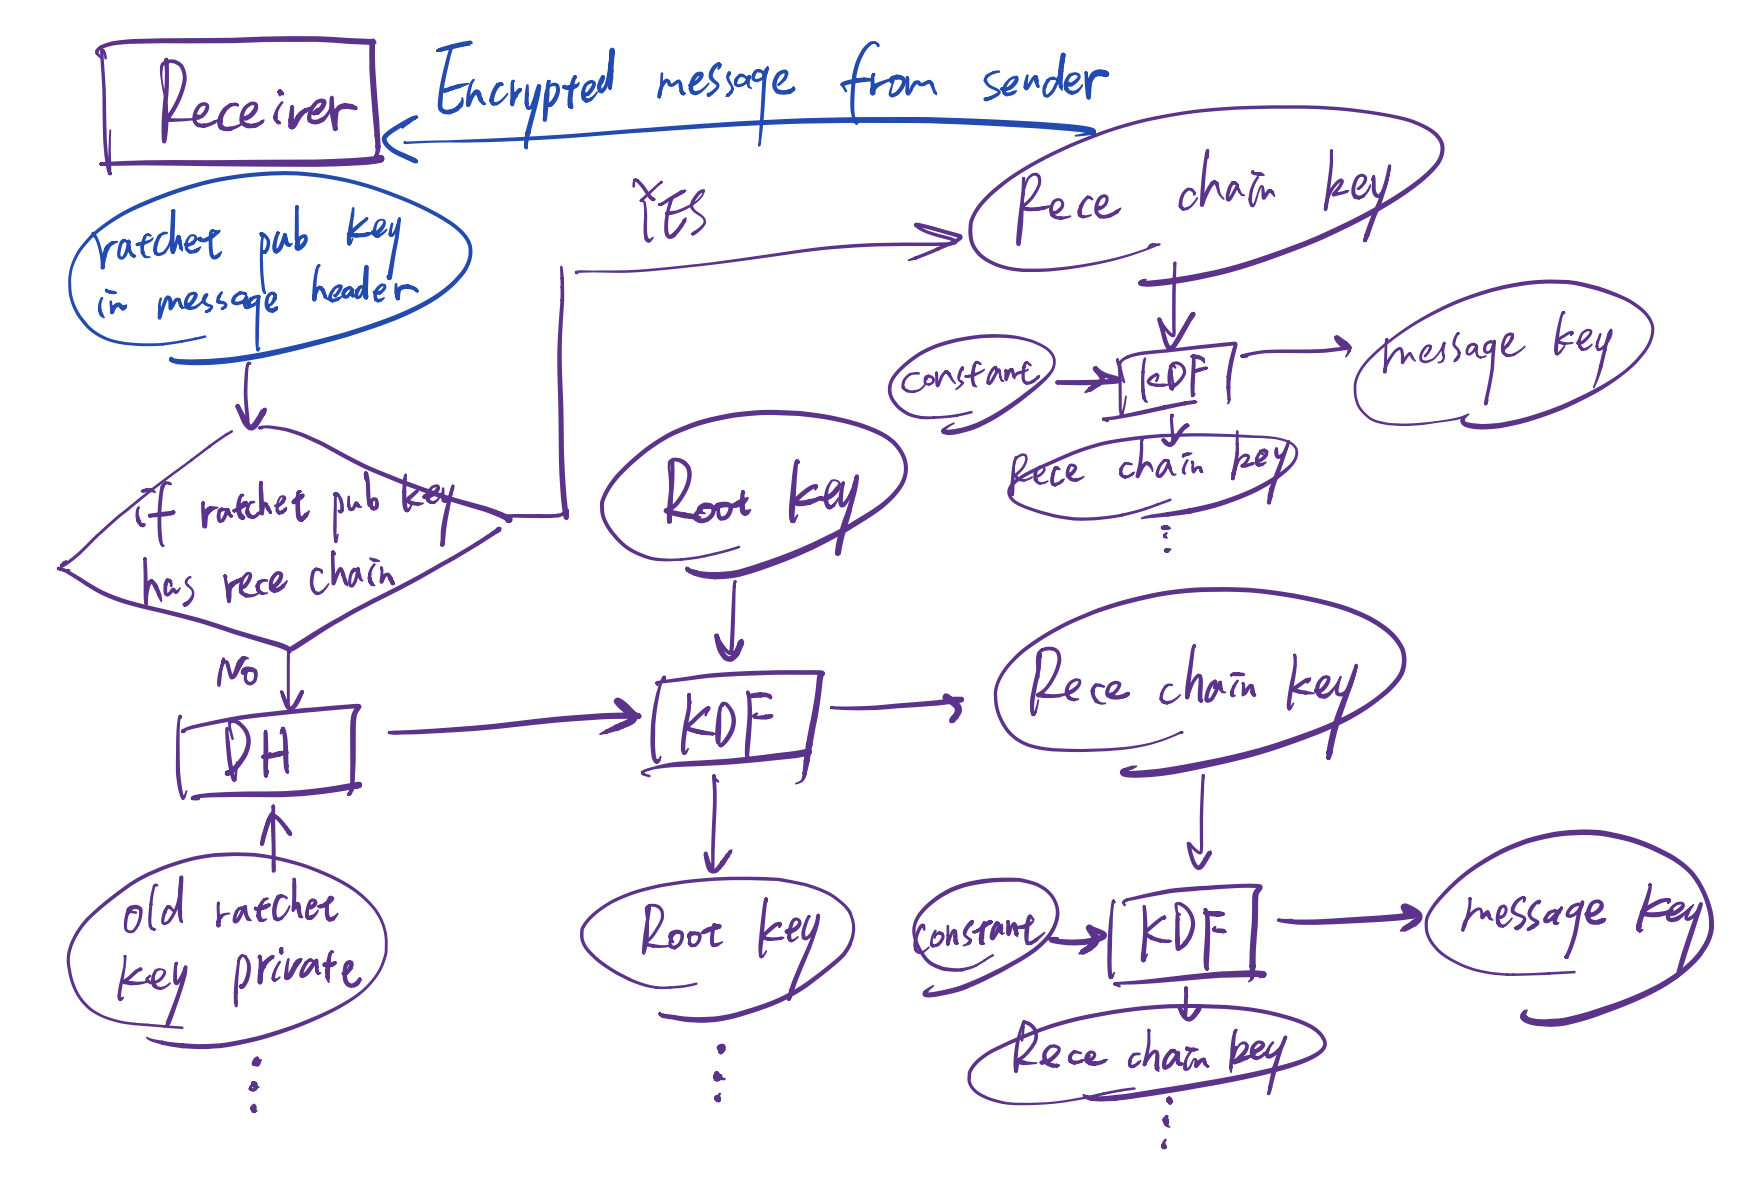
\includegraphics[scale=.5]{../3-Background/resources/DH-rece.png}\\
Figure 4.1: \textit{Implementing group chat by creating the pairwise chats between each other}
\end{center}

Fortunately, WhatsApp and Signal have already given the solution. Because of the high security feature of Signal Protocol in pairwise chat, members can exchange their chain keys via pairwise way. When the group chat is initializing, each member needs to generate a sending chain key as the second ratchet in Double Ratchet. Then they should use the pairwise chat to exchange their sending chain key with every other one in the group. After initialization, on each member's side there are only N-1 sending chain of others and one own sending chain. Every time the user wants to send some messages in the group, the user only needs to do a stepping on his own sending chain and get the correct message key for encryption which means one message only needs one encryption. For the receivers, they just need to find the correct sending chain corresponding to the sender and do the correct stepping to get the message key for decryption. This design is much better in time and space cost then the former. The figure 4.2 is the schematic diagram of it.

\begin{center}
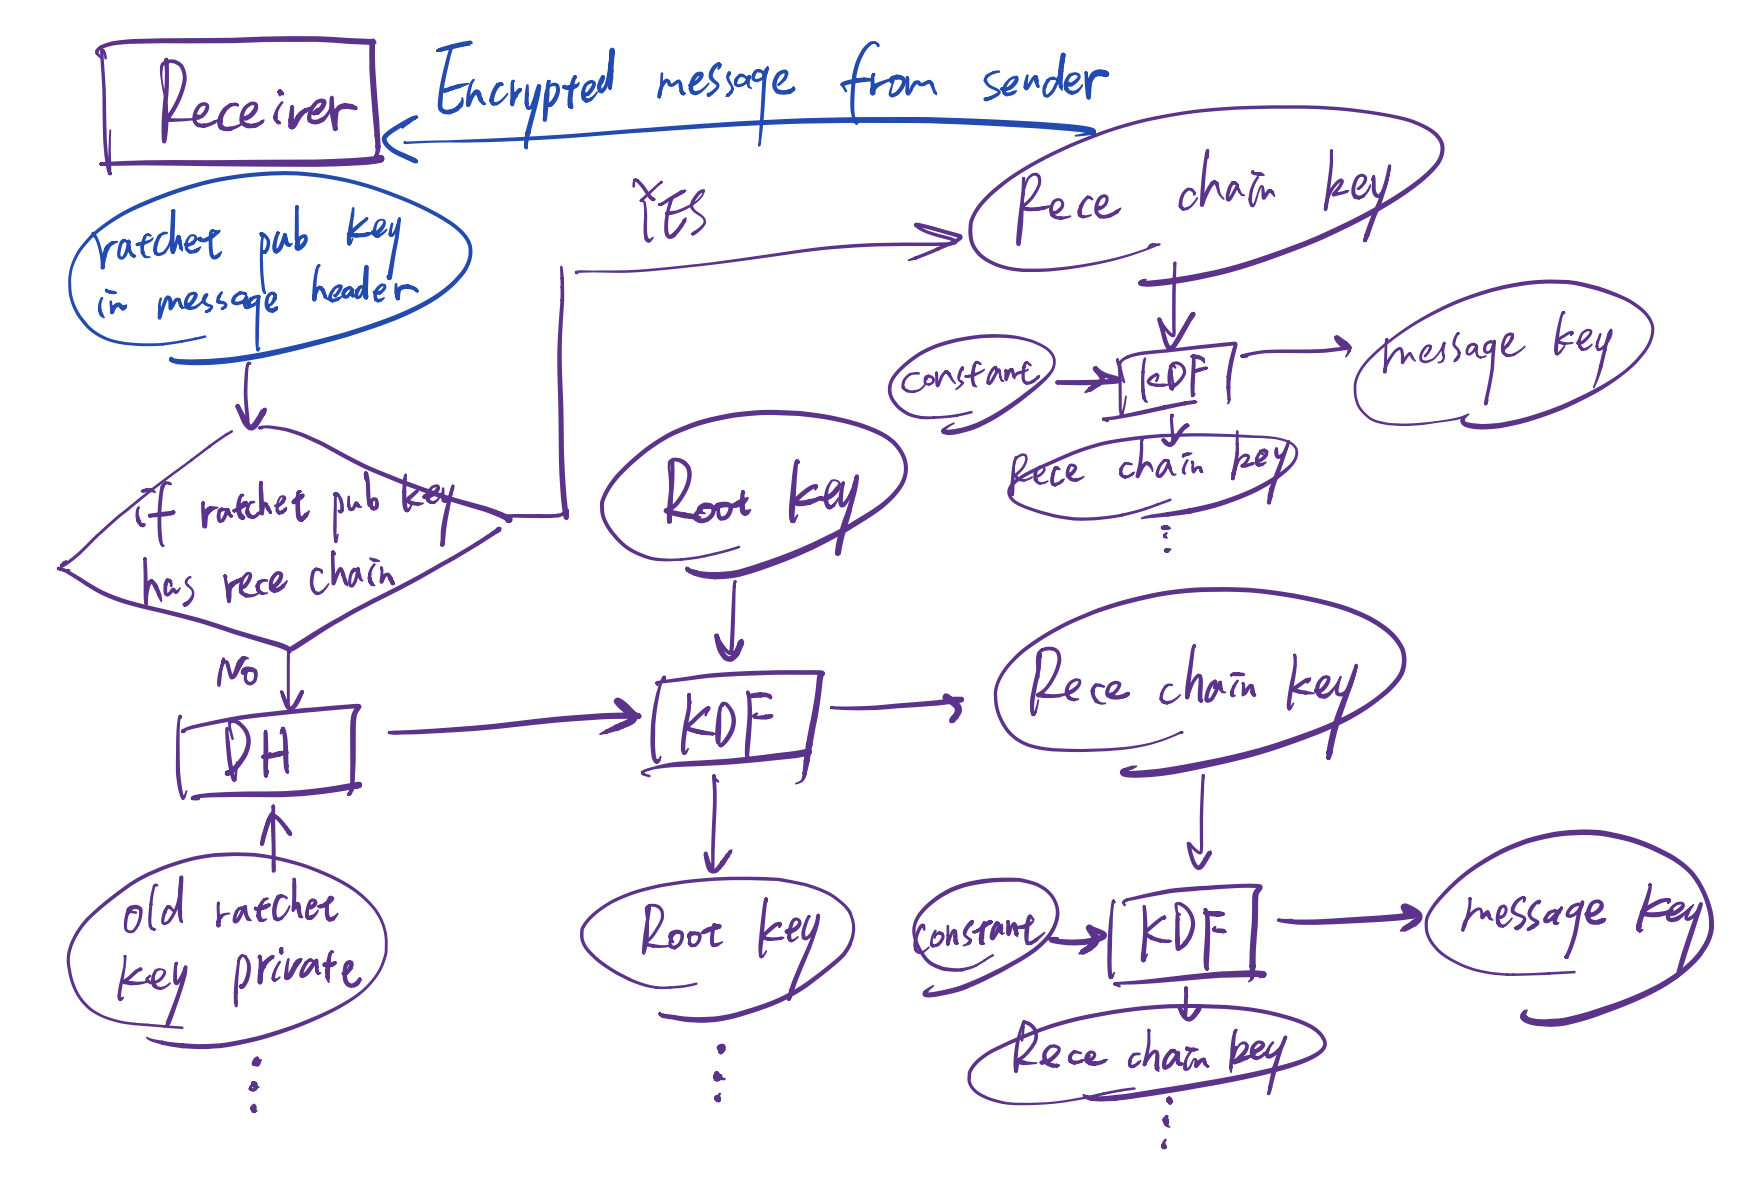
\includegraphics[scale=.5]{../3-Background/resources/DH-rece.png}\\
Figure 4.2: \textit{Implementing group chat by exchanging sender keys with each other}
\end{center}

\item Multi-device system

Switching device is an important function in a chat system. It allows users to get continuous using experience while changing their device. Because the Signal Protocol requires each account generates the unique key bundle for communication and the confidentiality of the private keys is the precondition of the chat's security. So to some extent, Signal Protocol is device-oriented. User's each device needs to generate a unique key bundle as a new account. In this system, there should be a new customize class User containing the username and deviceId fields, which means one user can have several accounts with same username but different deviceId. The figure 4.3 shows the user information structure in multi-device system.

\begin{center}
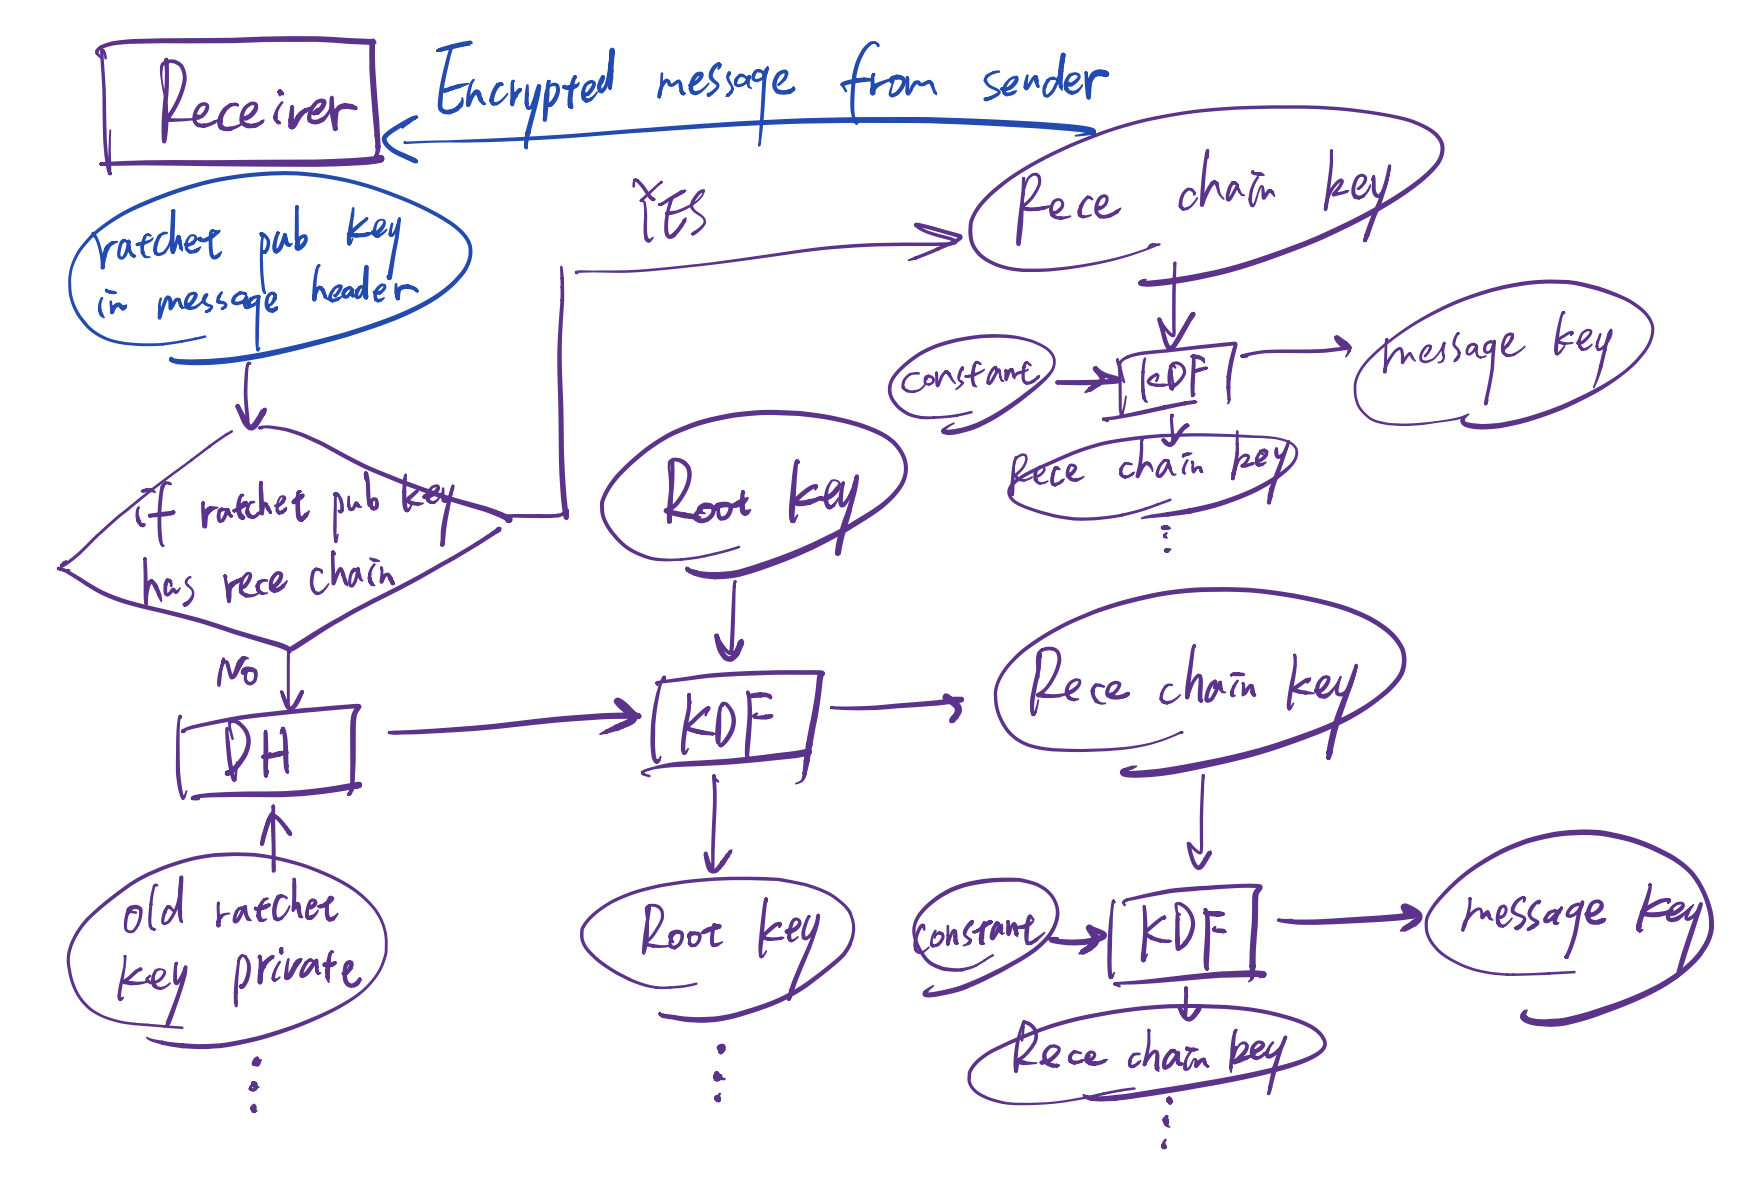
\includegraphics[scale=.5]{../3-Background/resources/DH-rece.png}\\
Figure 4.3: \textit{The user information structure in multi-device system}
\end{center}

When the user switch the device at the first time, it's necessary to register a new account with the same username and password but different deviceId. The requirement of the same password is to prevent adversaries' malicious registration. In the meanwhile, the new account generates a new key bundle and upload it to the server for further communication. The login function is also asked to change: the user's login information should include username, password and deviceId for the server to judge if this account is registered.

Once the user successes to switch the device, the old pairwise chats and group chats related to him on other's client side are still not updated. The messages from others are forwarded to the old device so that the user cannot receive the corresponding messages from others. To solve this problem, the system decides to inform all users when the user is switching device. Users will judge if there is any chat related to the switching user and update the switching user's information and key bundle from server if yes.

To avoid other users to send messages to the old account, the client will be inoperable while updating the switching user's information and key bundle. Once the client completed the update, users can send messages as before.

The update of switching user's information can be considered in two situations. In the pairwise situation, if there is corresponding session related to the switching user in Signal's session store, users need to request the switching user's key bundle of new account from server and update the chat session's member information. The alteration in group chat situation is relatively complicated. First users need to find the related group chats that contain the switching user in group members. Then they are supposed to generate a new sender key for later group communication. The reason for this operation is to guarantee the future security of group chat, because the switching user's old device maybe lost and exploited by the adversary to get later communication data if not changing each member's sender key. After generated the new sender key, users need to distribute it to every other one in the group chat as initialization. Users may do not initialize the pairwise chat with the switching user's new device, so before distributing the sender key, they need to initialize the pairwise chat to create a secure connection with the new device. Then the encrypted sender key can be delivered to the switching user's new device for further group chat. On switching user side, the user will judge if there is corresponding own sender key related to this group at the moment of receiving other's sender key. And the user will generate and distribute the new sender key if no. After all these operations, the group chat can work with the switching user's new device as before.

As for the consideration of message backup, the multi-device system adds a field variable named active while login. The user could only have one active account at the same time. If the account which is logging in was not active previously but would be active now, the multi-device system would update user's active account information to complete the device switch operation. When the account which is logging in was inactive previously and would not be activated now, the account could send the backup messages to the active account of the user. The figure 4.4 has an overview about the login handle in multi-device system.

\begin{center}
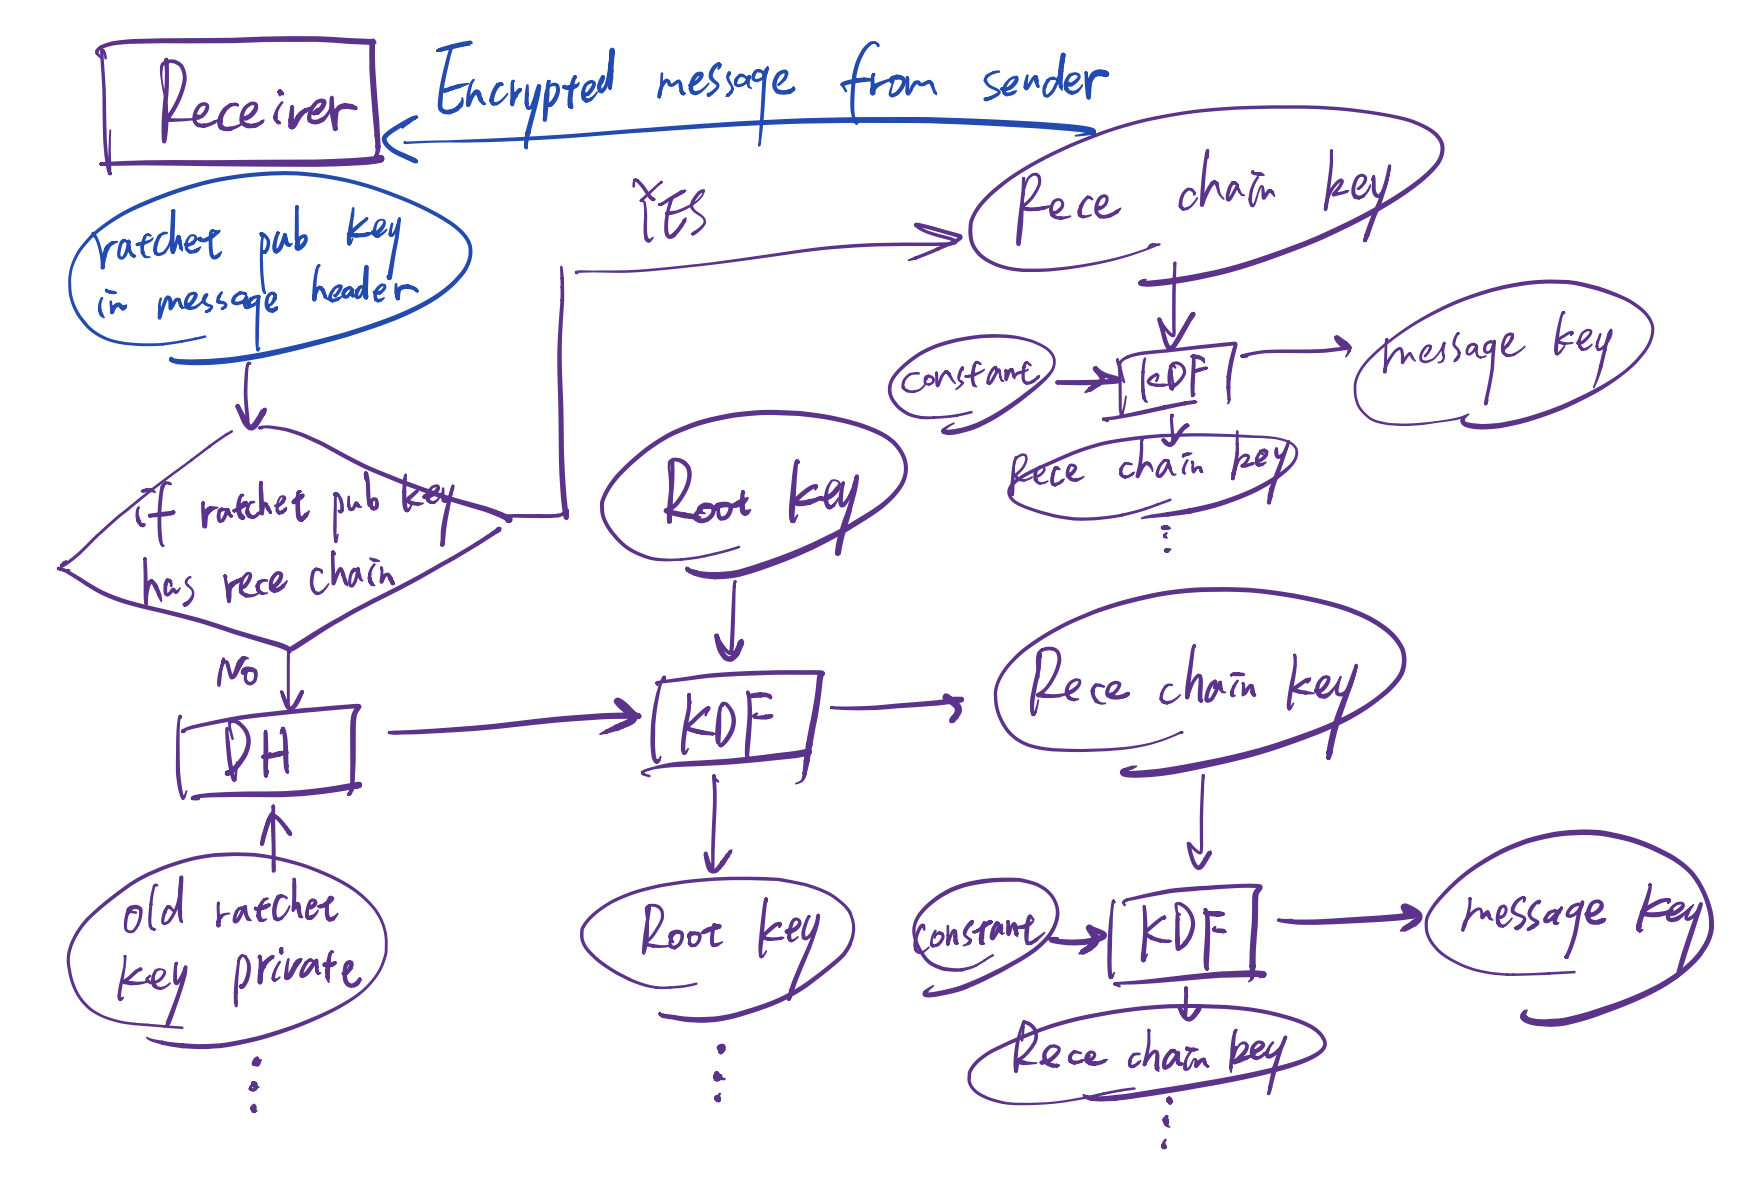
\includegraphics[scale=.5]{../3-Background/resources/DH-rece.png}\\
Figure 4.4: \textit{The login handle in multi-device system}
\end{center}

\item Chat fingerprint verification

The guarantee of Signal Protocol's security is that the both parties are indeed themselves. The secure pairwise chat can be monitored via MIMA (Man In The Middle Attack). As a simple example, the server serves as the adversary and wants to monitor the communication content between two users called Alice and Bob.

At the initializing time, Alice requests Bob's key bundle from server. However the server responses its own key bundle to Alice. Once the Alice completed the ratchet steps and encrypted messages, the members in this pairwise chat is Alice and server in fact. Then the server uses the Signal Protocol to decrypt the encrypted messages from Alice and establishes a secure pairwise chat with Bob using its own and Bob's key bundles. After that, the server encrypts the plain text from Alice again in the chat containing Bob and delivers it to the Bob. Until now, the server has two secure connections with Alice and Bob respectively and can decrypt the messages between them easily without their knowledge.

The key to solve this problem is how to ensure the two parties are the same in their perspective. In both parties' perspective, this pairwise chat's members should be Alice and Bob. However, on Alice's side the members of this pairwise chat are Alice and the server, on Bob's side the members of it are Bob and the server in fact. So comparing the two chats' identifiers is a good solution to check whether they are hijacked. The pairwise chat's fingerprint is generated using two parties' public identity keys and can be presented by a series of bytes. The two parties can compare own chat's fingerprint with the other's fingerprint via other communication ways but not the same pairwise chat. Because if they still use the previous pairwise chat to exchange their fingerprints, the server can replace the content of fingerprint for confusion. Once the users find they are monitored by adversary in pairwise chat, it's essential to update sender keys in all related group chats too. To reassure users that the server is not monitoring their communications, Signal Protocol is not used on server side in this system, but this function is still useful to prevent MIMA from adversary.
\end{enumerate}
\subsubsection{Server}
The server's duty in this system is responding to users' requests and forwarding users' messaging packages. 

In login and sign up functions, the server needs not only verify user's username and password, but also judge if the deviceId is registered or existing due to the alteration of User class.

The server is also required to respond to user's key bundle requests. Once received the key bundle requests, the server will inquire the key bundles from database corresponds to the userId.

In order to match Signal Protocol's asynchronous feature, the server is supposed to be designed to work in asynchronous. For example, Alice wants to send some encrypted messages to Bob who is offline currently. The server cannot find Bob in current online users list and stores the messages in cache. Once the Bob logins at some time, the server will load all related messages and send them to Bob as soon as possible. After that, the server will delete sent messages in cache to release the memory. This caching strategy is also applied to sender key distribution, switch inform and backup messages etc.

In the logout function, since the client stores history messages at local, there is no need for the server to handle it any more. The server's only duty in this function is informing other users which one is logging out.
\subsubsection{Database}
There are only two tables in the database, the Users table and KeyBundles table. To be compatible with the multi-device system, the User table is required to add a new field deviceId. The KeyBundles table contains the key bundles associated with corresponding users. Since the history chat data is not saved in database any more, the ChatData and Session table can be dropped. Figure 4.5 presents the table structure of Users and KeyBundles tables.

\begin{center}
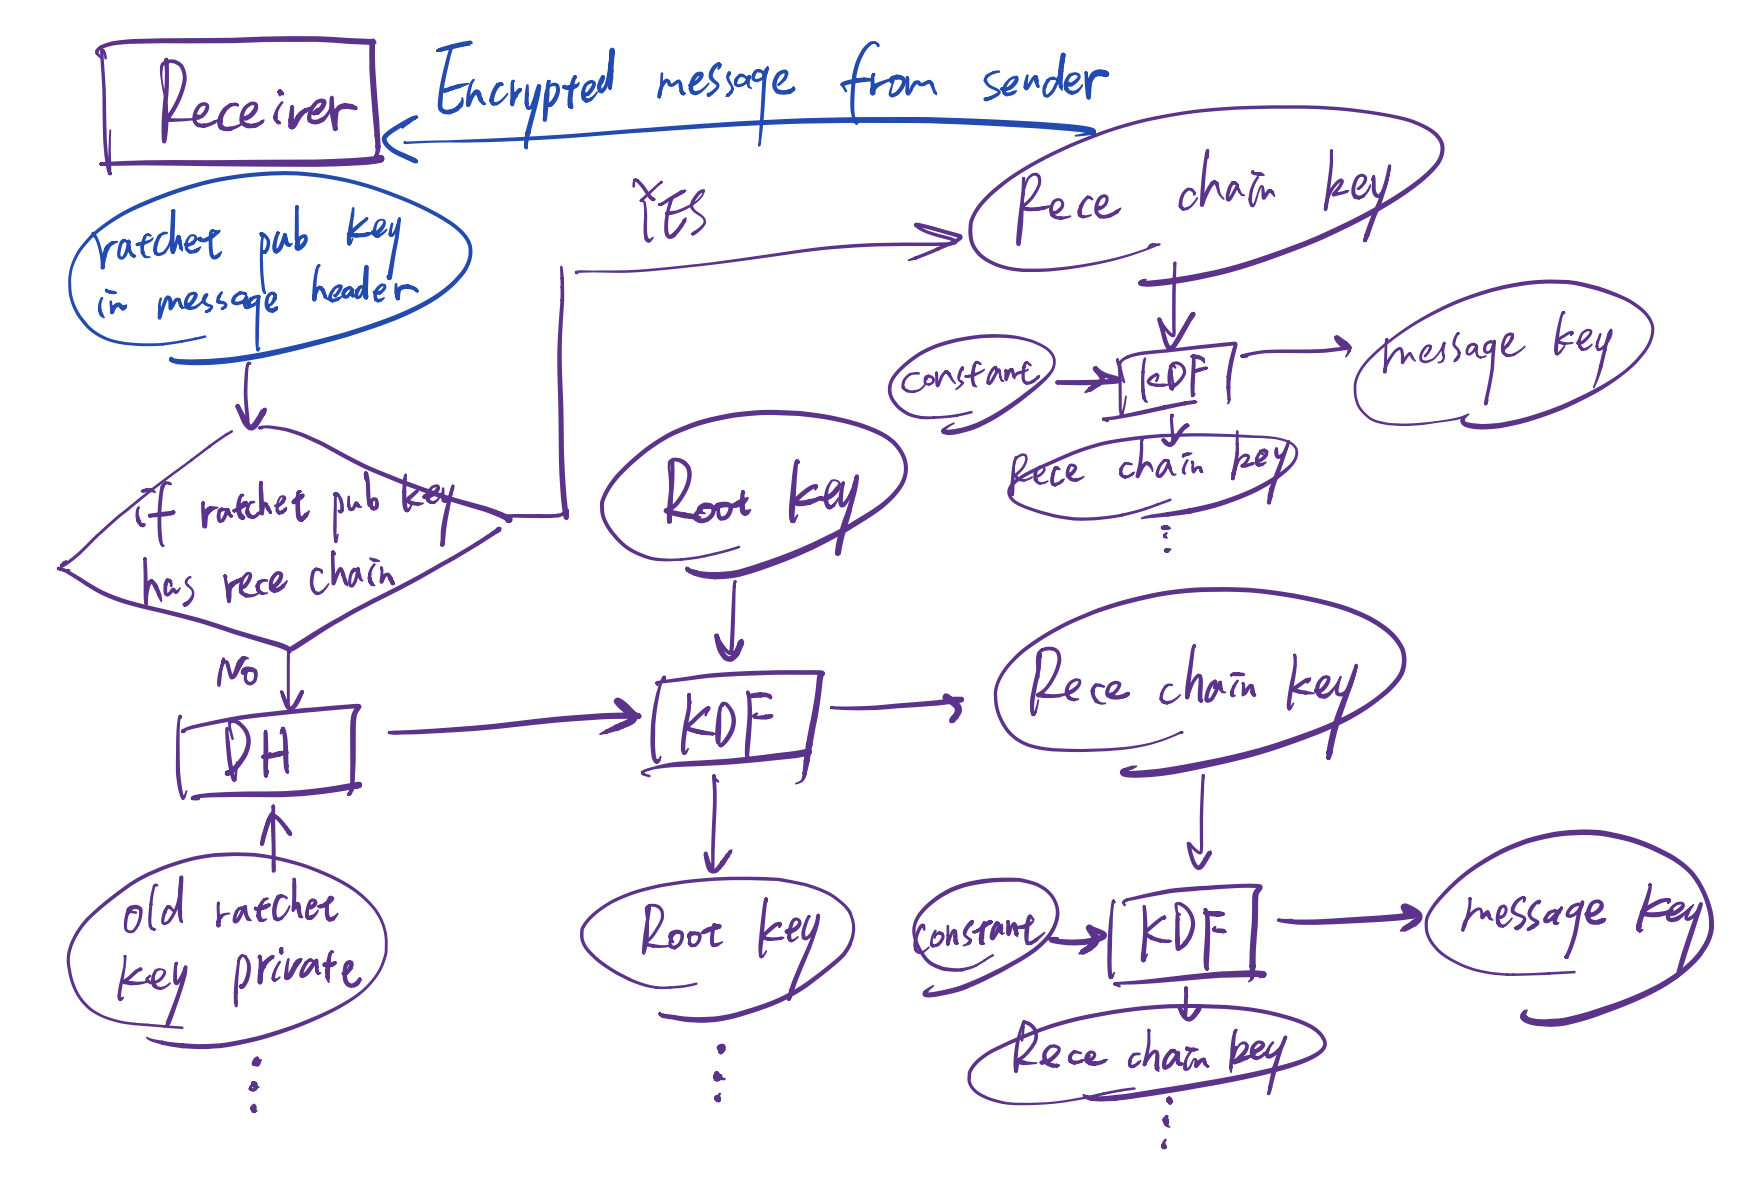
\includegraphics[scale=.5]{../3-Background/resources/DH-rece.png}\\
Figure 4.5: \textit{The structure of Users and KeyBundles tables}
\end{center}

\subsection{Implementation and testing}
The concrete implementation in this project can be divided into three main parts including the client, server and database. The first few sections will describe the implementation details and the justifications on corresponding side. The last section introduces the testing strategy and presents some testing examples of the whole system.
\subsubsection{Implementation in Client}
The main work in the client includes the implementation of Signal stores, development of pairwise chat and group chat, updating session information while devices switching and the verification of pairwise chat fingerprint. All the Signal related behaviours are put in the EncryptedClient and EncryptionHandler class such as the creation or load of Signal stores, encrypted chat initialization and message encryption.

\begin{enumerate}[label=(\roman*)]
\item Implementation of Signal stores

The libsignal-protocol-java lib provides several Signal store interfaces for developers to implement. There are all kinds of ways to implement them. These stores keep the Signal related states including identityKeyStore, signedPreKeyStore, preKeyStore, sessionStore and senderKeyStore.

Each store maintains other users' certain public keys. For example, identityKeyStore maintains other users' identity keys, signedPreKeyStore maintains others' signed pre keys. The data structure storing related keys that the implementing class used is HashMap. Map is a suitable data structure to save the KV pair. In these Signal stores, the key and value in the KV pair is the account and their keys respectively. HashMap is an efficient implementation of Map, since there is no need to order keys in Signal stores, using HashMap can improve the accessed speed.

Once determined the data structure of storage, the implementation of constructor, setters and getters is more easier. After constructing the Signal stores, the user needs to add their own signed pre key and pre keys in SignedPreKeyStore and preKeyStore respectively. Otherwise the user cannot recognize their own keys in further session's initialization.

Besides, developer can add some other functions in the implementing stores such as serializing the keys in the storage and judging whether there is any related session in sessionStore. All the functions related to the Signal stores can be implemented in them to keep the code in Object-Oriented style.

\item Development of pairwise chat and group chat

The core functions during the chat are initializing the chat and encrypting or decrypting the messages.

During pairwise chat initialization, once received the key bundle from the server, the client will invoke the pre-packaged functions in Signal lib to create a corresponding session. Then a sessionCipher that used for further encryption and decryption can be generated via Signal lib's function. The same situation in group chat is relatively complicated. When the user wants to create a new group chat, the client will invoke the initGroupChat function. In this function, the client will generate a new sender key for this group chat and judge if there is anyone who has not created a pairwise chat before. After establishing secure communication with all other members, the client will start to invoke the distributeSenderKey function to encrypt and distribute its own sender key to others. In the meanwhile, the client is also supposed to handle others' sender keys -- storing them in the senderKeyStore's HashMap for further decryption. Then a pre-packaged class from Signal lib called groupCipher can be generated for further encryption and decryption. JavaFx will generate a waiting alert to make the client inoperable during the initializing process until the client's own sender key distributed. Because if the group messages delivered before the sender key, the receiver cannot decrypt them with the correct sender key.

While communication, the client can invoke sessionCipher's encrypt or decrypt function from Signal lib to secure the chat content. The encrypt function is wrapped in EncryptionHandler class for both pairwise and group chat invocation. The output of it is serialized to bytes for the transmission convenience.

\item Session update while devices switching

For the continuity of the chat, the client is required to update related session members' information while the user is switching device. Once the client received the switching inform from the server, it will check whether there is any related pairwise chat or group chat immediately. Judging the related chat session in history chat data is not reliable, because the pairwise connection may be established while the group chat initialization but there is no chat session record in history data. The wiser choice is using the sessionCipher and senderKey to judge if there is any related session needs to be updated.

The client will request the user's key bundle of new device to reinitialize the pairwise chat and generate a new sender key which will be distributed to others to reinitialize the group chat.

During these processes, the client invokes javaFx's function to generate a waiting alert to make the application inoperable. The reason for it is to avoid users to lost the messages before the switching completed.

\item Pairwise chat fingerprint verification

To help the users to figure out whether they are monitored while communicating, the client has the function getFingerprint according to the pairwise chat parties. The function constructs a pre-packaged class from Signal lib called NumericFingerprintGenerator and invokes the createFor function to generate the fingerprint of pairwise chat. There is a button on the head of the chat, once the user clicked it, the client will use javaFx to generate a information alert which shows the fingerprint string for user's comparison.
\end{enumerate}

\subsubsection{Implementation in Server}
The functions that are required to be implemented can be listed as three parts: response to users' requests, storage of undeliverable messages and user identify verification.

\begin{enumerate}[label=(\roman*)]
\item Response to users' requests

To construct a Signal compatible server, the server is supposed to have the ability responding the users' Signal related requests. For example, the users will request other's key bundle while initializing the pairwise chat and send their sender key to the group members.

This system uses socket programming to implement the communication between the server and the client. There is a common class on both server and client side called ConnectionData representing the package data during connection. This class must be same on both sides or it will be serialized to the bytes that the other side cannot deserialize. Both client and server process the data reception by an independent thread. Once the party received a connectionData, it will deserialize the connectionData first and then do some operations corresponds to the type of data. The figure 4.6 presents the structure of ConnectionData and the process of communication between the server and client.

\begin{center}
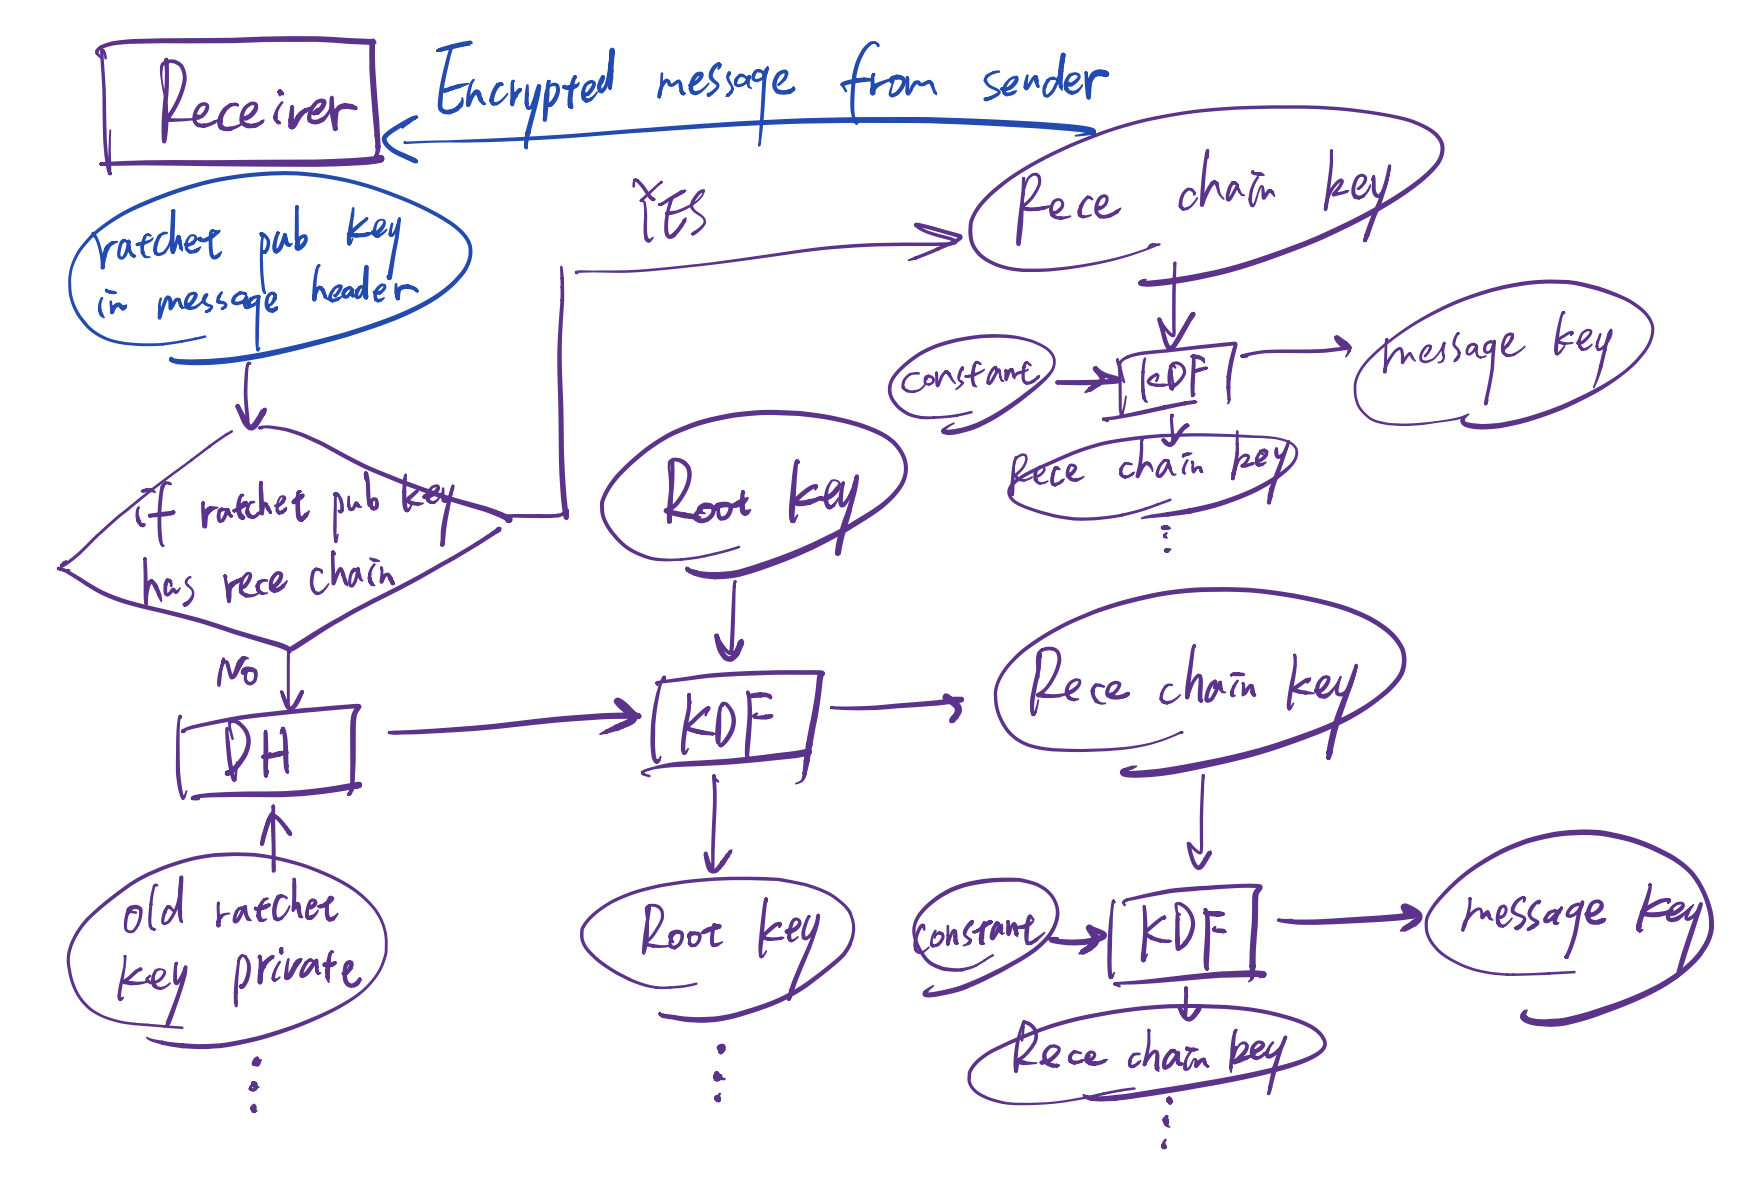
\includegraphics[scale=.5]{../3-Background/resources/DH-rece.png}\\
Figure 4.6: \textit{The process of communication between the server and client}
\end{center}

The ability of responding the user's key bundle request is essential in a Signal system. The server adds a new filed variable in connectionData named keyBundle to represent the key bundle payload and defines the type of this kind of connectionData. While processing the key bundle request, the server would inquire the certain key bundle from the database by associated userId. If the key bundle is not found according to the given userId, the server would throw an IllegalArgumentException for alerting.

Other functions of responding to user's requests are almost the same as the key bundle request function. Because the I/O architecture in both server and client is synchronous, sometimes the communication between the server and client is quite complicated for development. For an instance, while reinitializing the group chat due to the device switching, there may be several situations needed to be handled, the following steps are required to be written repeatedly in every situation branch. In some processing scenes, the server uses package combination strategy to solve this problem. For example, the server would combine all the key bundles together in one response when the user requests several users' key bundles at one time.

\item Storage of undeliverable messages

Storing the undeliverable messages in server's cache is an essential solution for asynchronous messaging environment. Sometimes the messaging receiver may be offline so that the server cannot deliver the messages correctly. In this situation, the server would store the messages until the receiver is online again, then send and delete them.

For the implementation of this function, the server maintains several storage including depositPairwiseData, depositSenderKeyData, depositGroupData, depositSwitchData and backUpMessages. The data structure that these storages used is HashMap which can store the KV pair efficiently. In the first four storages, each user account corresponds to an ArrayList containing the related connectionDatas. In the last backUpMessages, each user account corresponds to another HashMap containing the history backup.

Every time the server processing the package forward, the server would try to get the outputStream according to the user account first. If there is no related outputStream, the server would put the message in the corresponding storage's HashMap with related user account. Then while every user's login, the server would traverse all the storages to get the associated messages and deliver them to the user. In the getting deposit data functions, the deletion operation at the end is essential or the user would get the same message again in further login.

\item User identify verification

After implemented the multi-device system, the user identify verification needs alteration too. The information of user is expanded by a new filed variable: deviceId. In the initial design, a user could have several accounts with the same username and password but different deviceId. In the meanwhile, a user could only have one active account at the same time. The active account is the account that others' messages would be forwarded to. While switching accounts, the user could choose to activate the account or not. If the user activates the account which means the user switches the account normally, the server would inform all the others to update the session information. If not, the user can login to that account without activation for message backup.

So the verification of user identify should consider the username, password, deviceId and activation. In the login situation, the server would inquire the records of given username, password and deviceId. If the result set is empty, the verification is failed. Then if the activation's value is true, the server is required to update the user's active account information in database. 

In the registration situation, things are more complicated. First the server is supposed to check whether this account has been registered before by username and deviceId. The password filed is not used in this function for the security consideration. Then the server should judge if this account is a new user's account by checking whether the inquired result set is empty. If the registering account is not a fresh user's account which means the username used for registration has already existed in database, the server must verify the user's password to prevent adversary's malicious registration. After that, the server should set all the user's other accounts' activation to false because the active account is the new registered one. Finally, the server inserts the new account into database with associated information.
\end{enumerate}

\subsubsection{Implementation in Database}
In database, there are only two tables: Users table and KeyBundles table. The Users table's alteration is only adding a new field deviceId in it. The KeyBundles table is a new created table for users' key bundles storage. The KeyBundles table is formed by userId, registrationId, identityKey, preKeysId, preKeys, signedPreKeyId, signedPreKey and signedPreKeySignature. The most complicated problem is how to maintain all the preKeys and preKeysId of users. Creating a new table to store the preKeys of users is a little space and time consuming which would cause the performance problem. Because each preKey's length is confirmed to 33 bytes, all the preKeys of one user are combined to a whole series of bytes and the preKeysId is counted from 0. Every time the server loads the key bundle for user's request, 33 bytes of preKes bytes are sliced from the front and the preKeysId would be added by one. Due to this solution, the preKeys can be maintained with other key bundles in one table which decreases the server's access time.

\subsubsection{Testing}
The testing of this system can be divided into two parts: junit testing and black-box testing. The system uses junit5 to write the tests and the gradle can generate the testing report automatically.

The junit tests cover the functions including the Signal encryption, javaFx rendering logic and jdbc executions etc. All the junit tests are passed both in the server and client. Figure 4.7 and figure 4.8 present the testing reports generated by gradle in the server and client.

\begin{center}
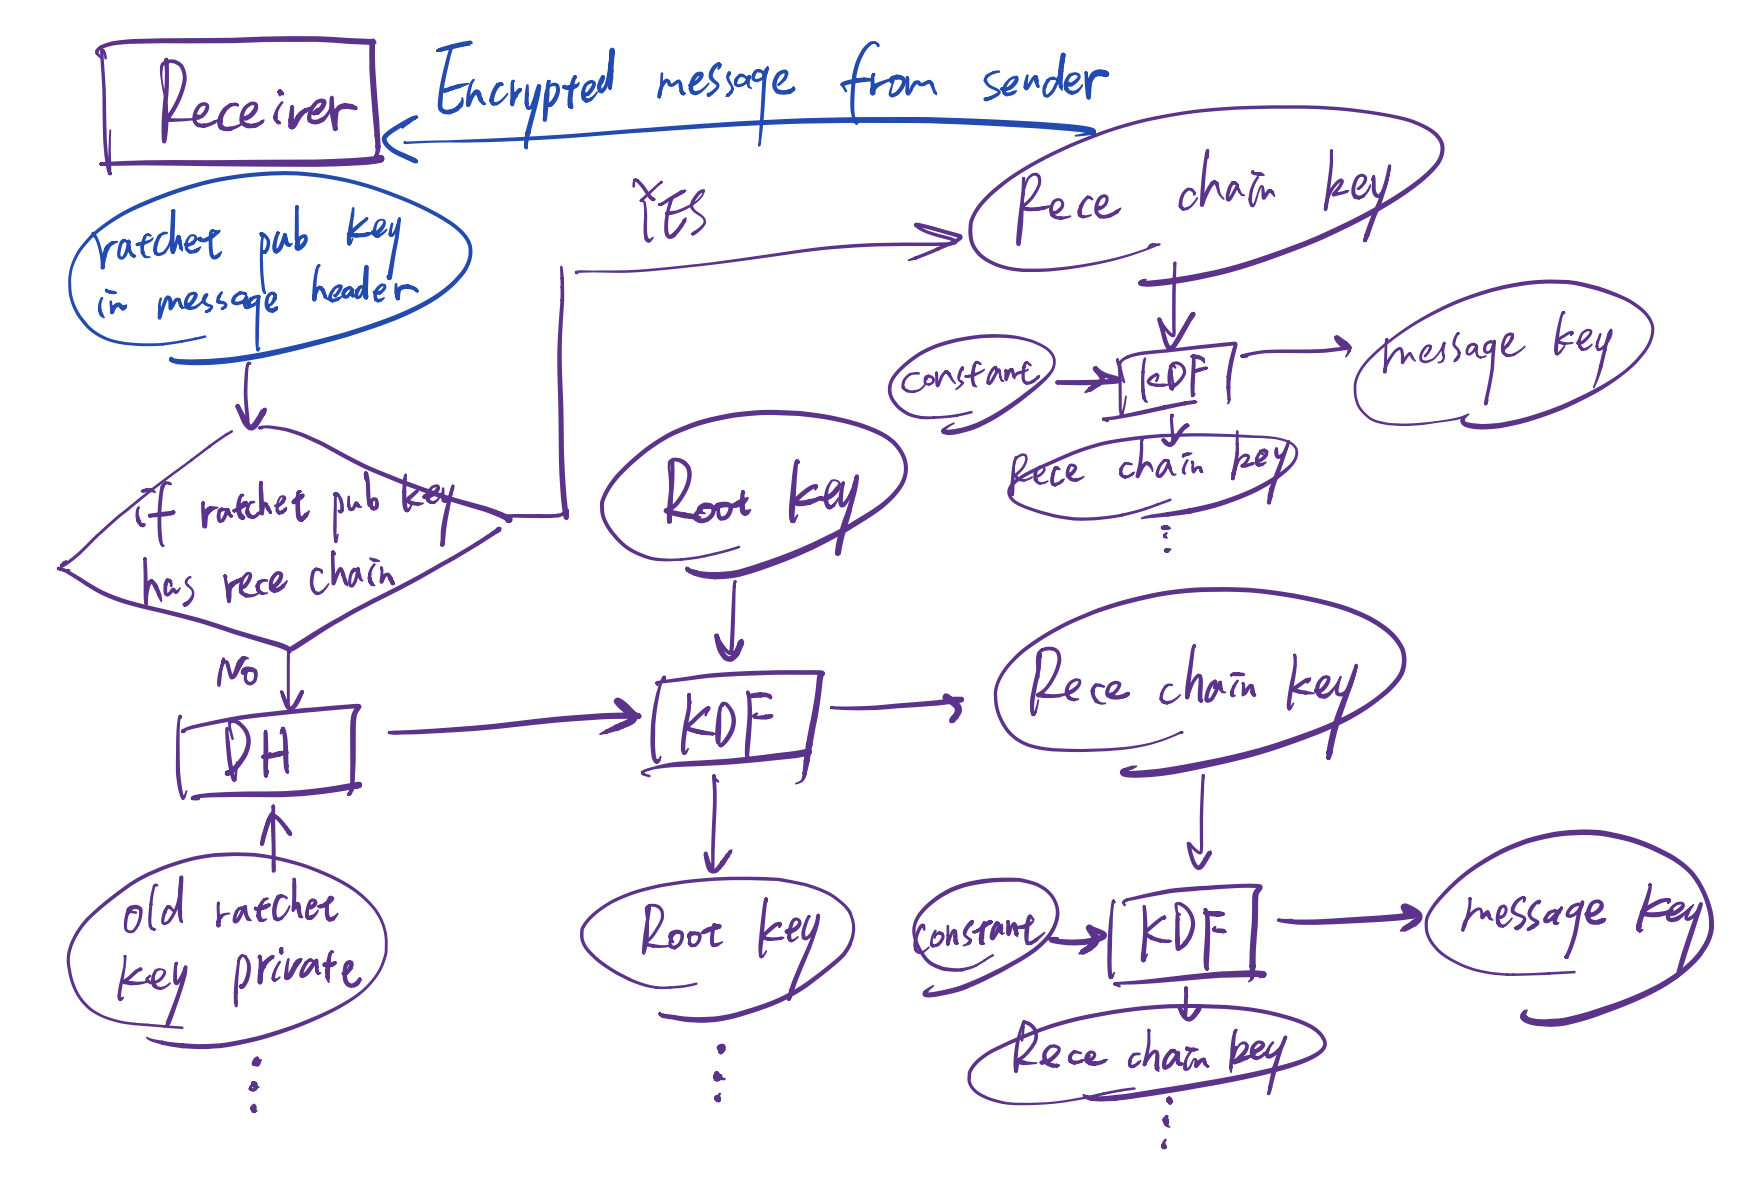
\includegraphics[scale=.5]{../3-Background/resources/DH-rece.png}\\
Figure 4.7: \textit{The testing report of junit tests in the client}
\end{center}

\begin{center}
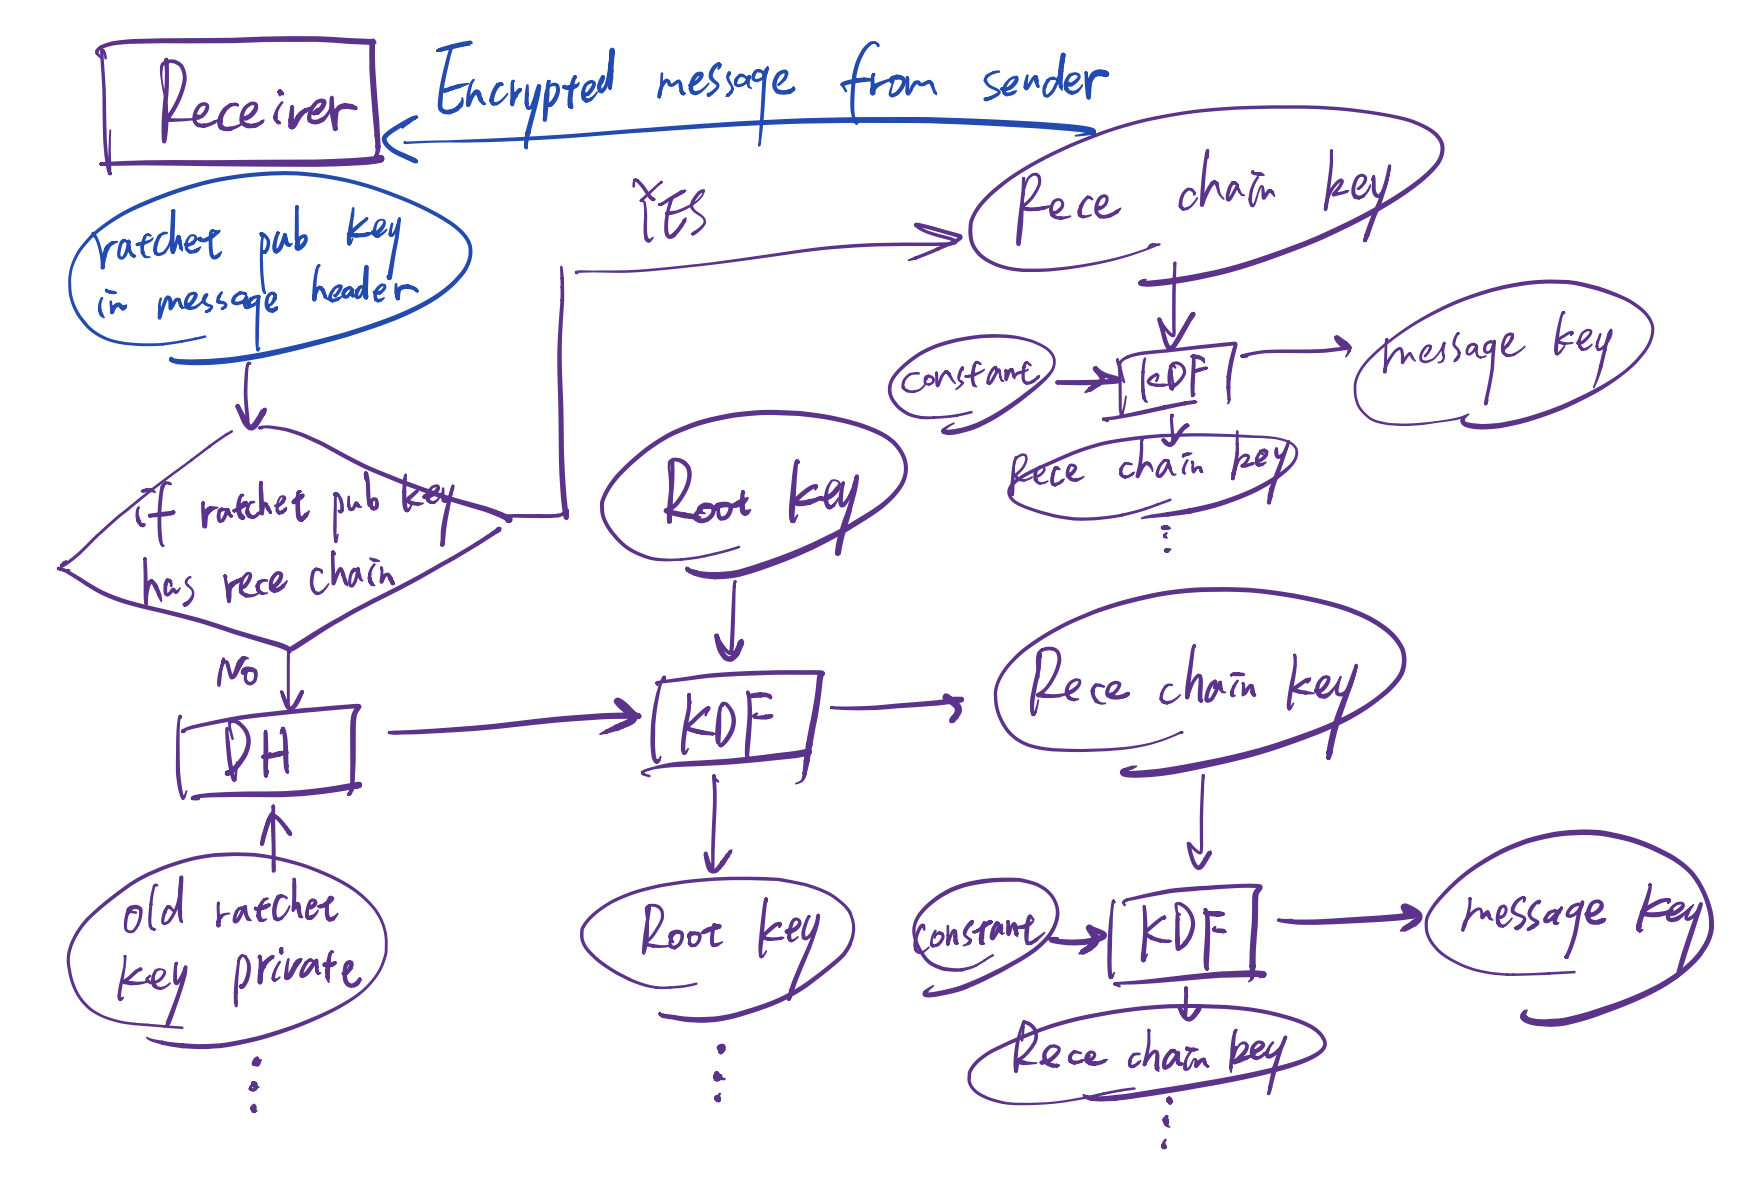
\includegraphics[scale=.5]{../3-Background/resources/DH-rece.png}\\
Figure 4.8: \textit{The testing report of junit tests in the server}
\end{center}

The black-box testing mainly tests the pairwise chat, group chat function and pairwise chat fingerprint verification. The situations includes the initialization, chatting and switching. The following parts present the result of different situations. Before all the testing, assuming there are three accounts called Alice, Bob and Cathy already been registered. The deviceId of them is 1 in default.

\begin{enumerate}[label=(\roman*)]
\item Pairwise chat testing

In the synchronous environment, Alice and Bob are both online. First Alice initializes the pairwise chat with Bob, after the shown of waiting alert, Alice could send messages to the Bob. The figure 4.9 and figure 4.10 present the initialization and chatting of pairwise chat respectively.

\begin{center}
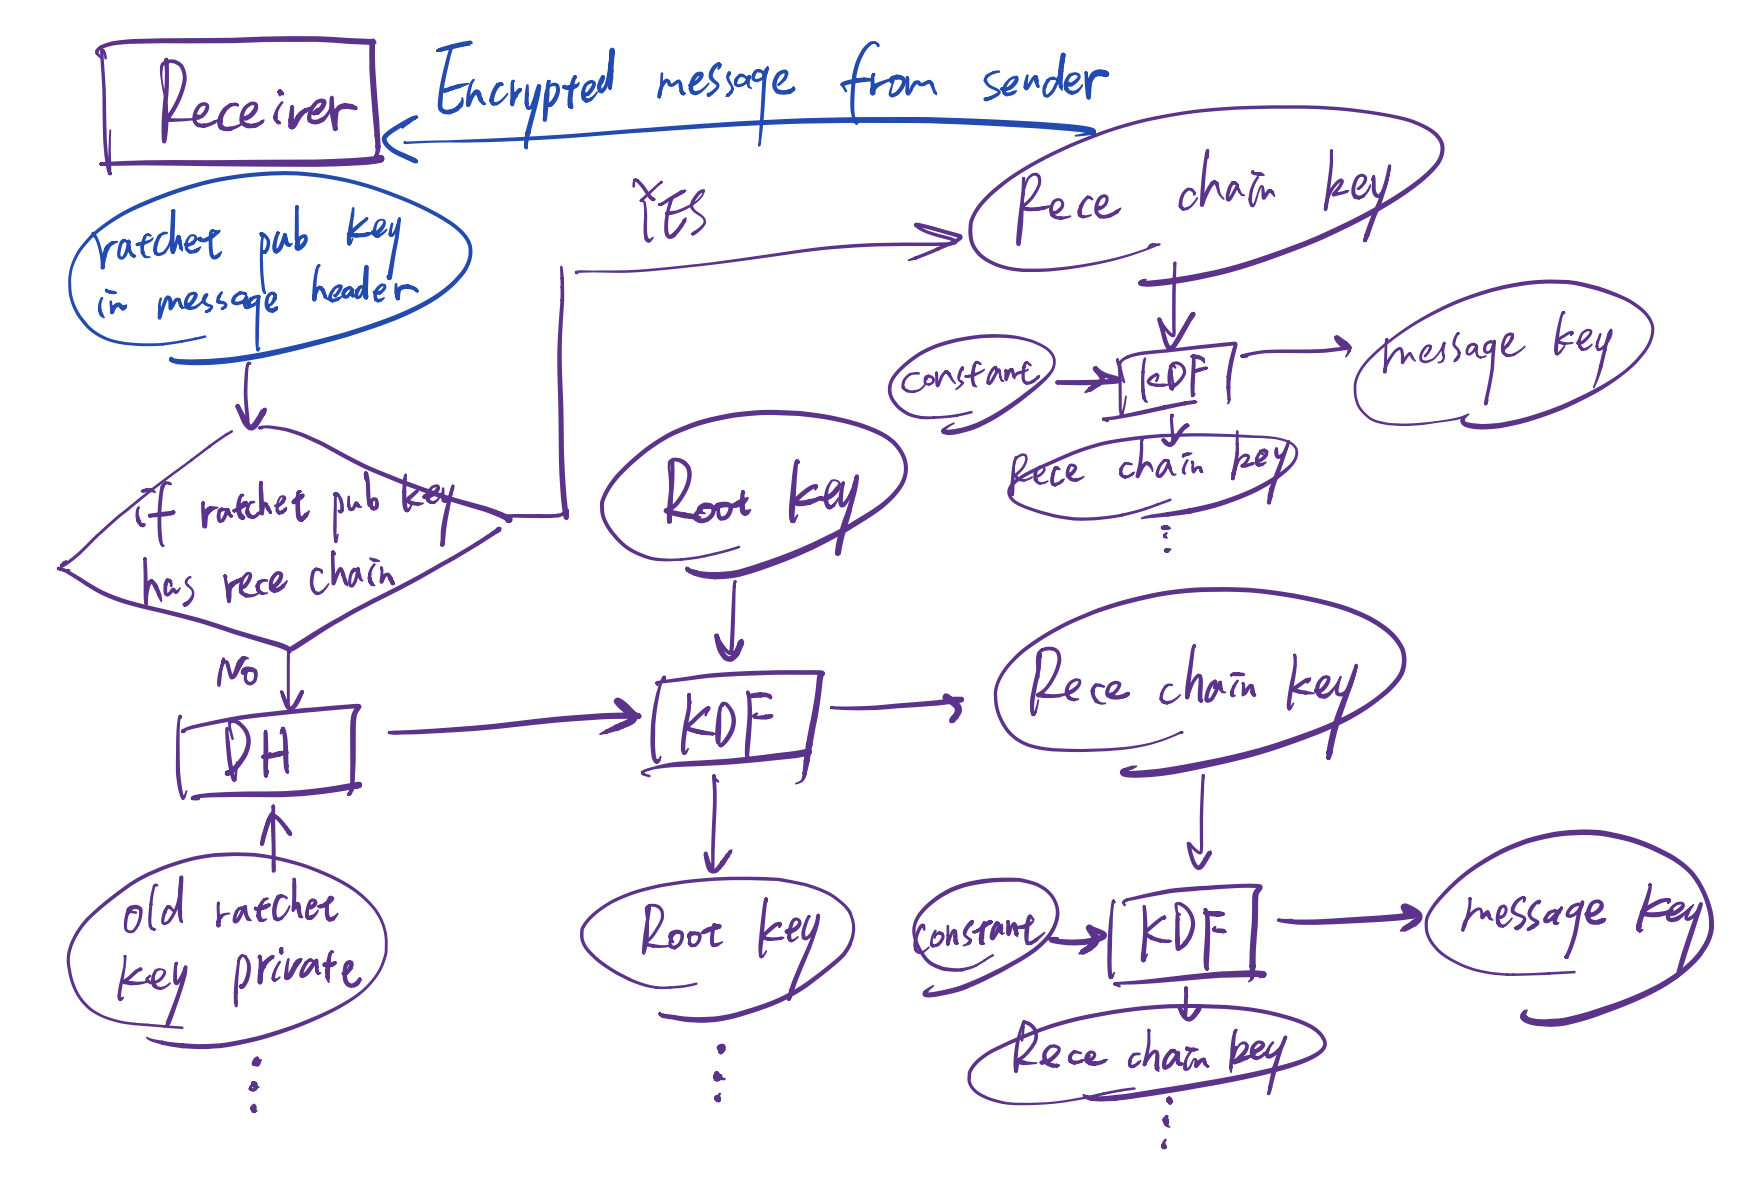
\includegraphics[scale=.5]{../3-Background/resources/DH-rece.png}\\
Figure 4.9: \textit{The initialization testing of pairwise chat}
\end{center}

\begin{center}
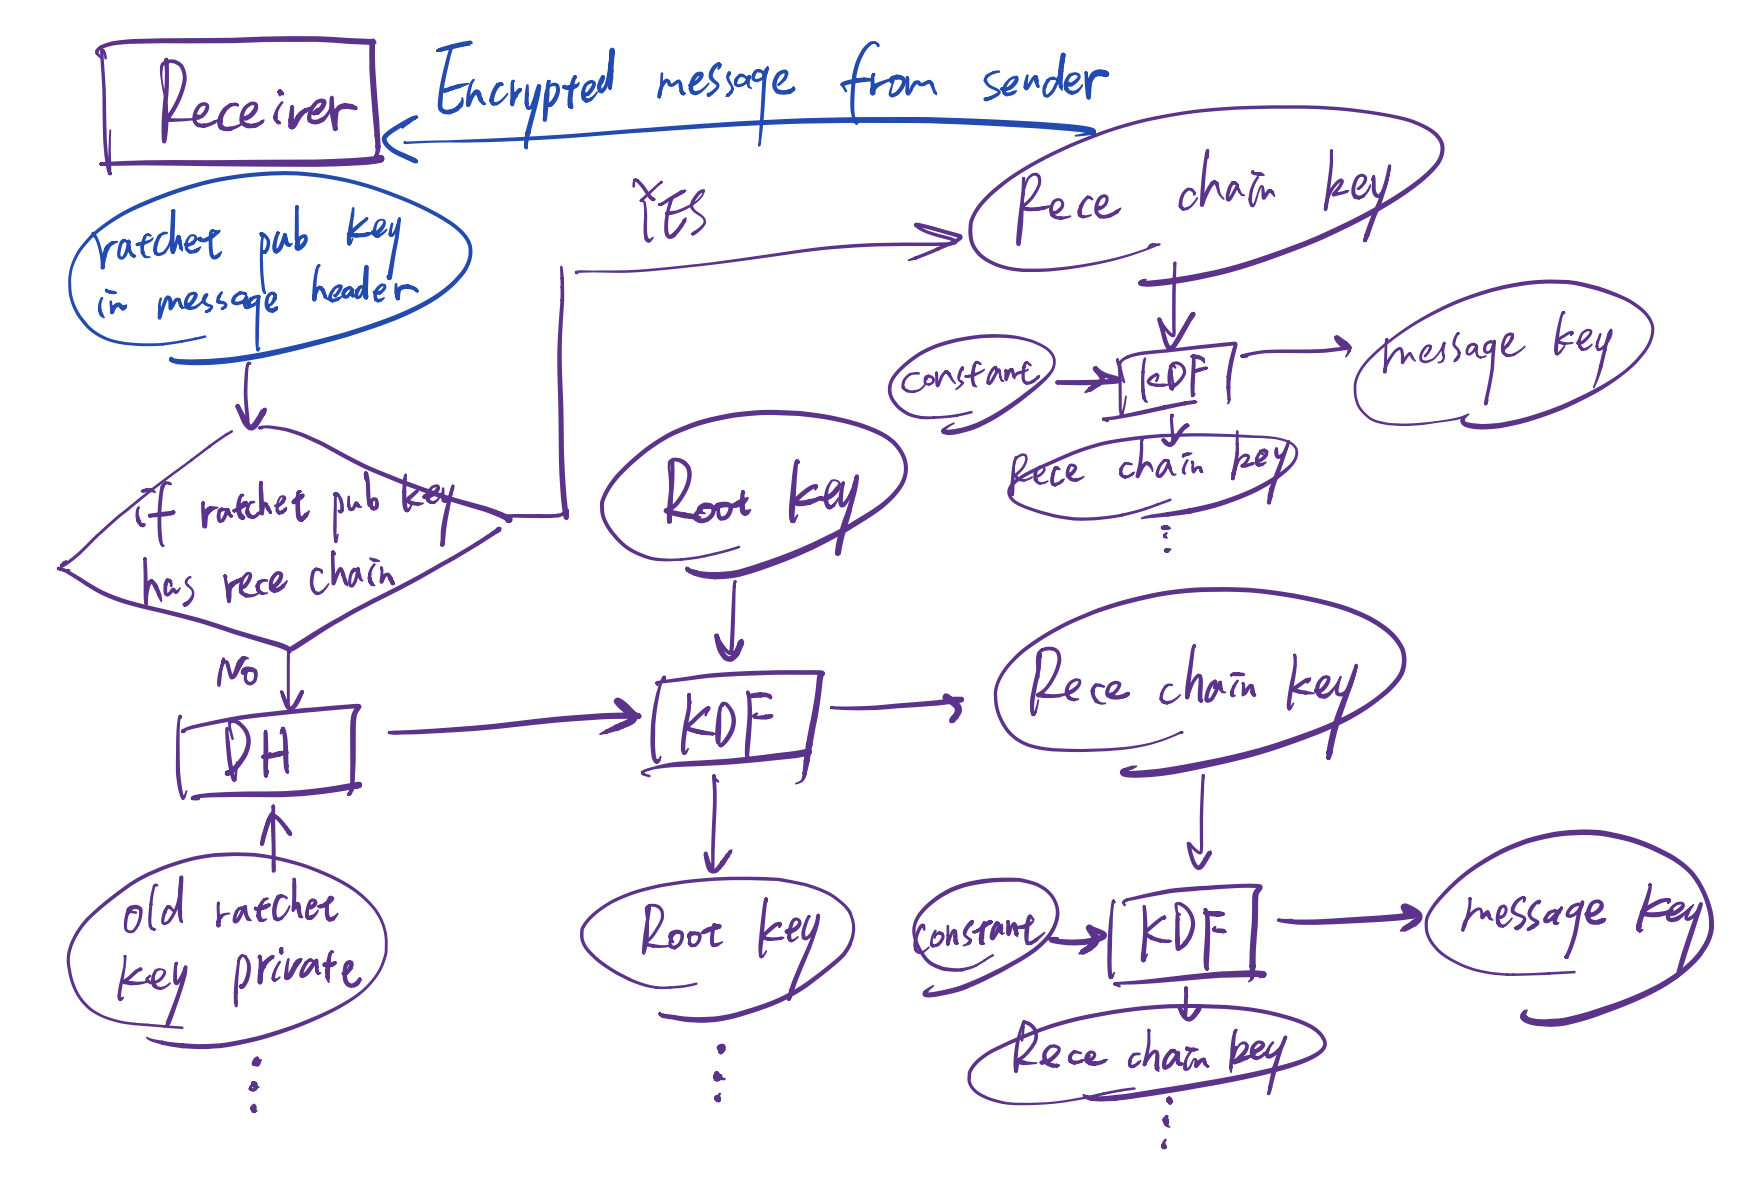
\includegraphics[scale=.5]{../3-Background/resources/DH-rece.png}\\
Figure 4.10: \textit{The chatting testing of pairwise chat}
\end{center}

In the asynchronous environment, only Alice is online while Bob is offline. Alice sends Bob some messages and see whether Bob gets the messages once login. After testing, the pairwise chat could work correctly in this situation. This testing also covers the tests of history message storage and Signal states storage.

\item Group chat testing

For the purpose of testing group chat in synchronous environment, Alice, Bob and Cathy are supposed to be online at the same time. While group chatting, the creator of the group chat Alice should request other's key bundles first for secure connection with them. Then generation and distribution of sender key is required. After the shown of waiting alert, Alice can send messages to the members. On Bob and Cathy sides, once they received the sender key from Alice, the initialization of the group chat starts in the meanwhile as Alice does. Then all the members could chat in the group. The figure 4.11 and figure 4.12 present the initialization and chatting of group chat respectively.

\begin{center}
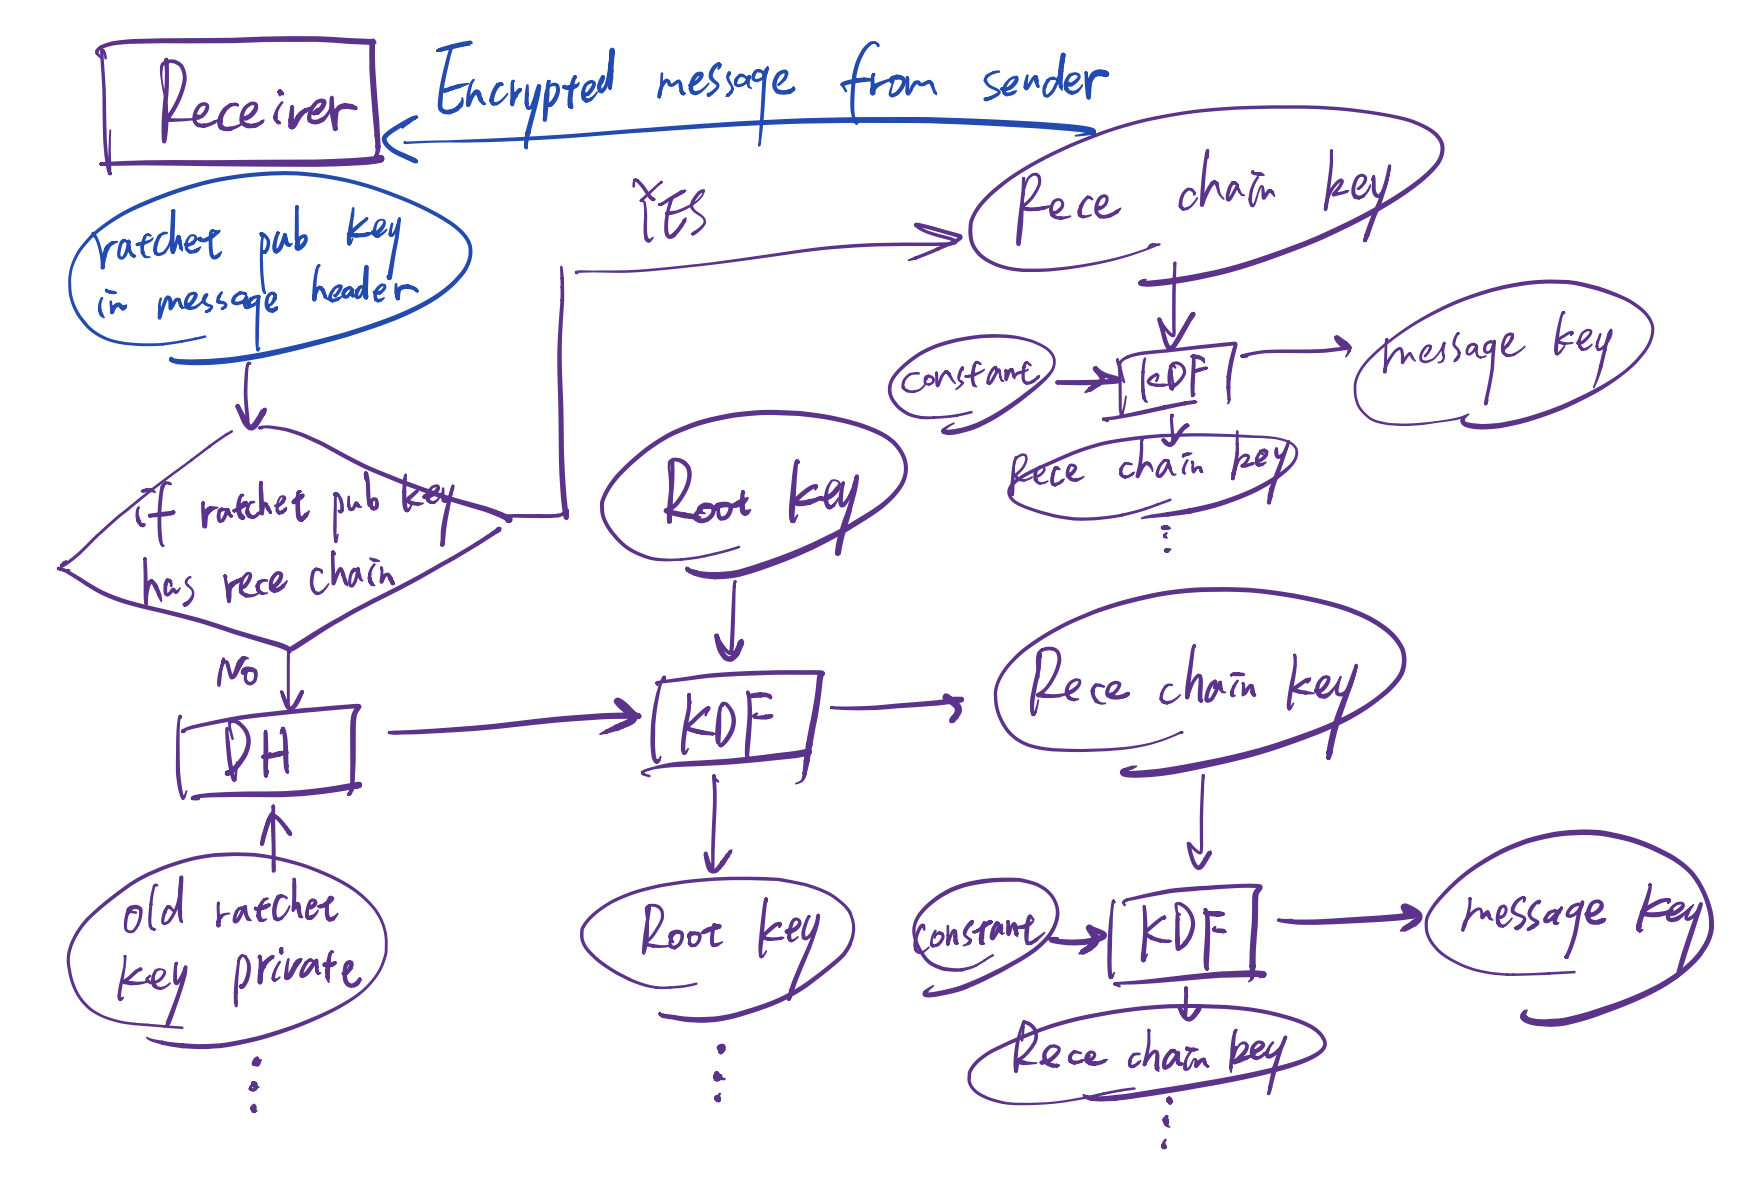
\includegraphics[scale=.5]{../3-Background/resources/DH-rece.png}\\
Figure 4.11: \textit{The initialization testing of group chat}
\end{center}

\begin{center}
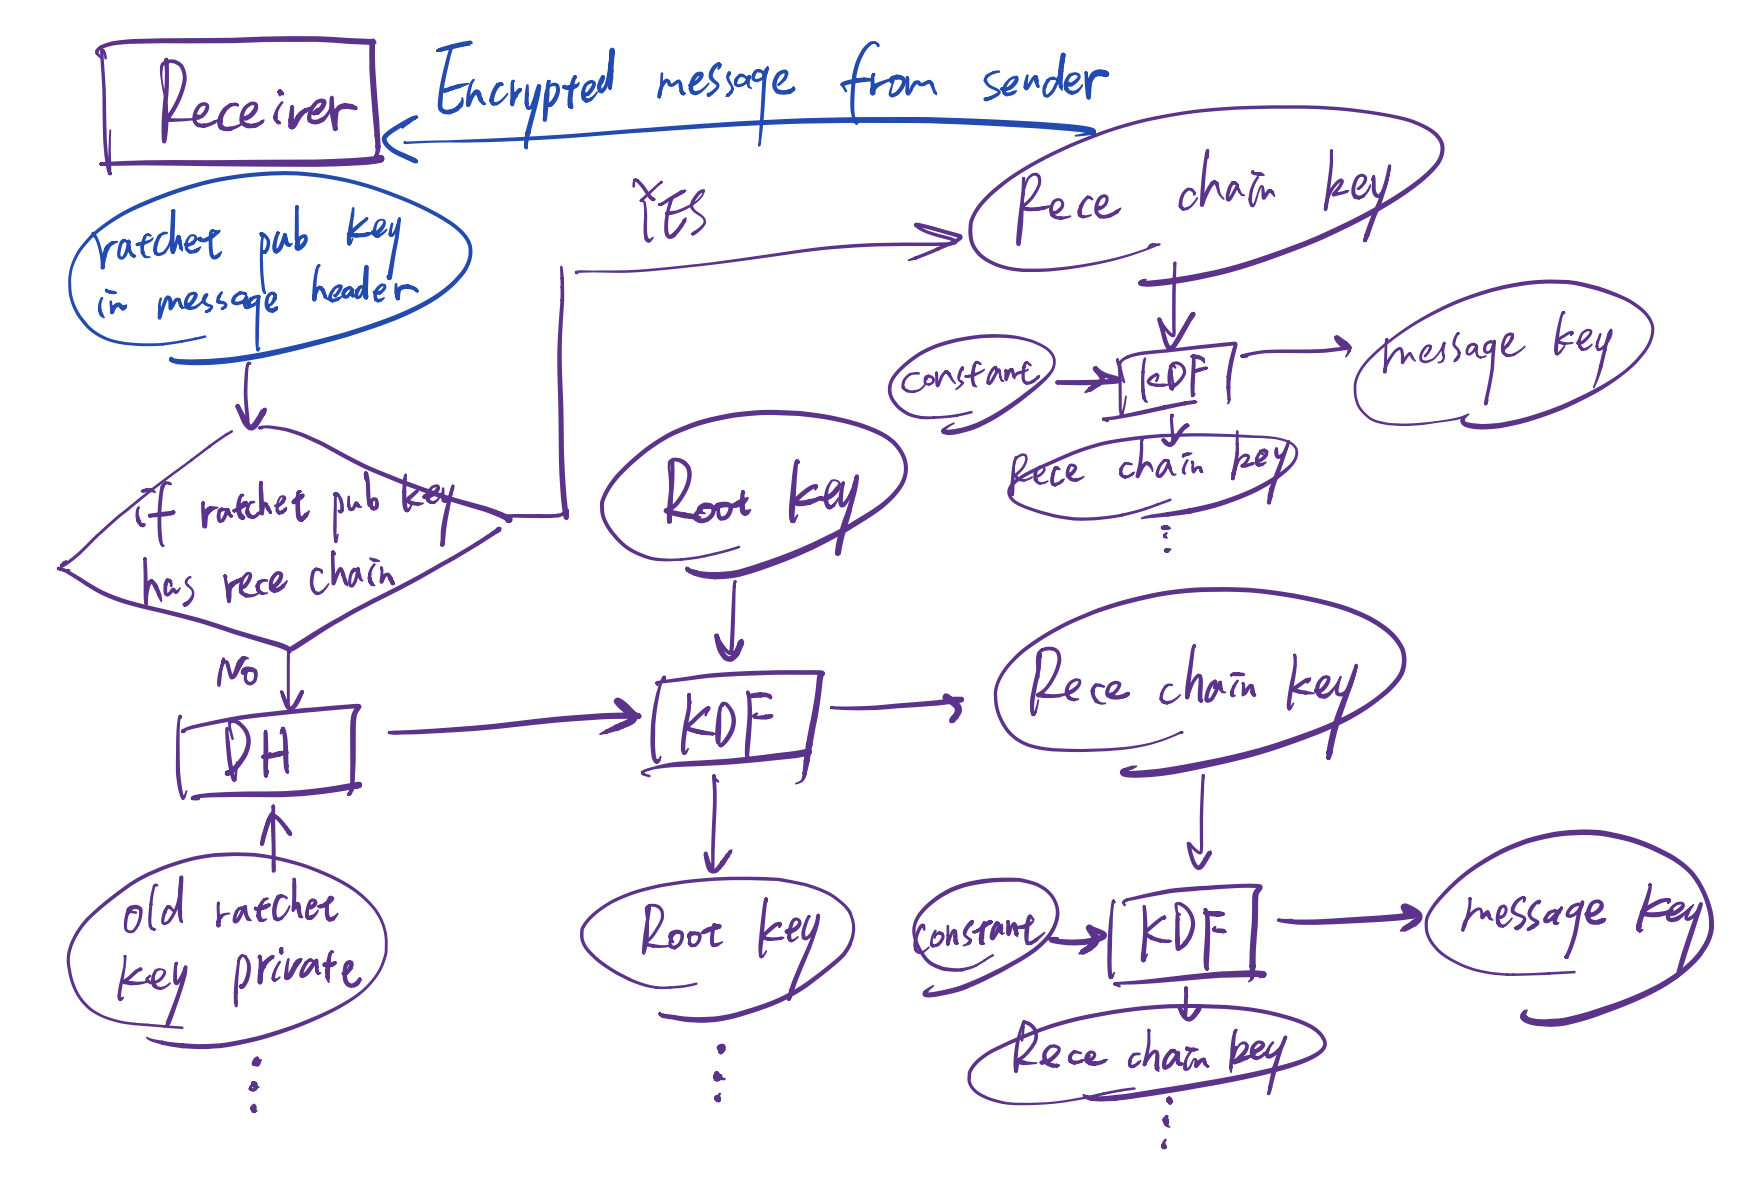
\includegraphics[scale=.5]{../3-Background/resources/DH-rece.png}\\
Figure 4.12: \textit{The chatting testing of group chat}
\end{center}

In the asynchronous environment, Cathy is required to log out first, Then Alice and Bob would have some chats during this time slot. Once Cathy login again, Cathy could receive the undeliverable messages and chat with members means the group chat could work as expected in the asynchronous environment.

\item Switch device testing

The stability of chat after switching device is essential in the multi-device system. To test if both pairwise chat and group chat could work correctly after switching devices, there is a pairwise chat and a group chat created already. Alice has a pairwise chat with Bob and a group chat with Bob and Cathy. First Bob is required to log out and register a new account with deviceId 2. After the reinitialization, both pairwise chat and group chat are supposed to work correctly including receiving and sending messages. The figure 4.13 and figure 4.14 present the reinitialization and chatting in this situation.

\begin{center}
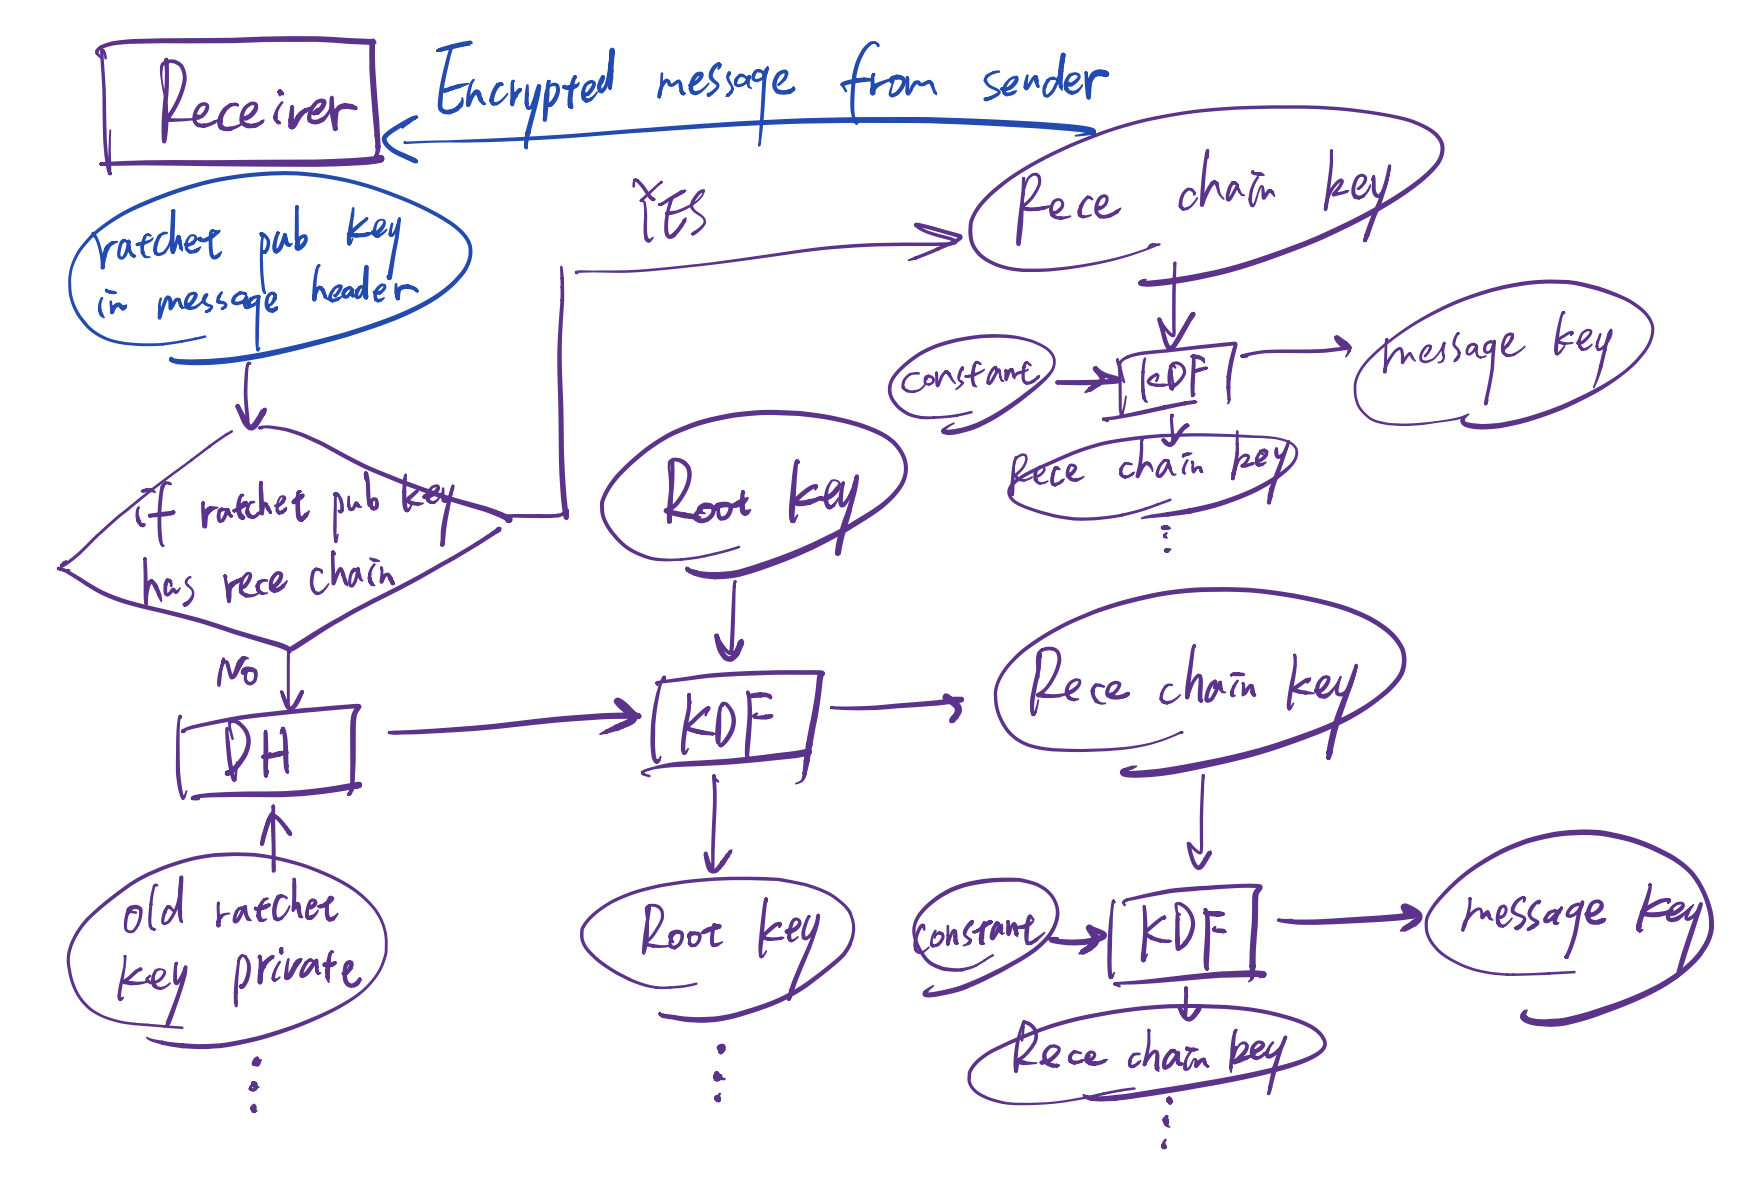
\includegraphics[scale=.5]{../3-Background/resources/DH-rece.png}\\
Figure 4.13: \textit{The reinitialization of group chat after switching the device}
\end{center}

\begin{center}
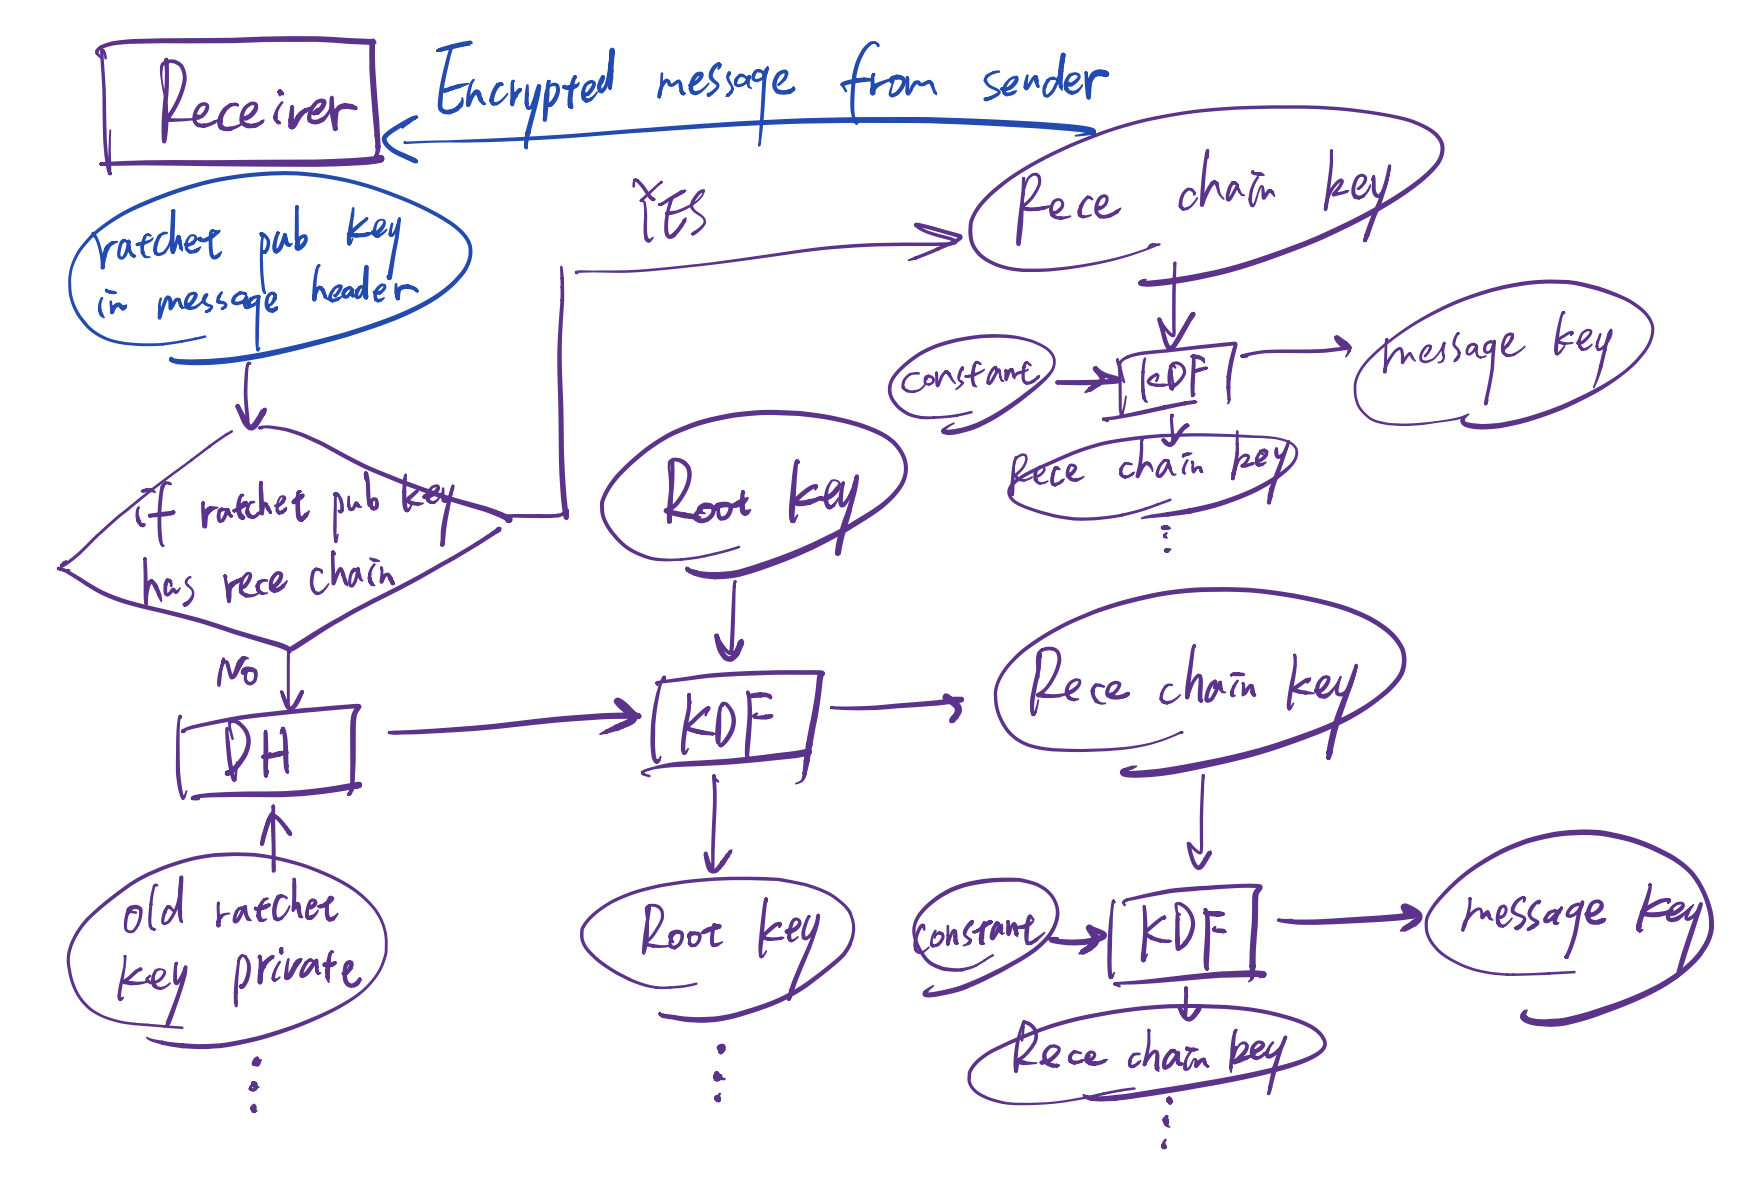
\includegraphics[scale=.5]{../3-Background/resources/DH-rece.png}\\
Figure 4.14: \textit{The chatting of group chat after switching the device}
\end{center}

\item Pairwise chat fingerprint verification

The testing pairwise chat fingerprint verification between Alice and Bob requires there is an already created pairwise chat between them. After clicking the verify button on both Alice and Bob sides, the information alert including the fingerprint of the chat is shown in the client. The figure 4.15 and figure 4.16 present the result of this function.

\begin{center}
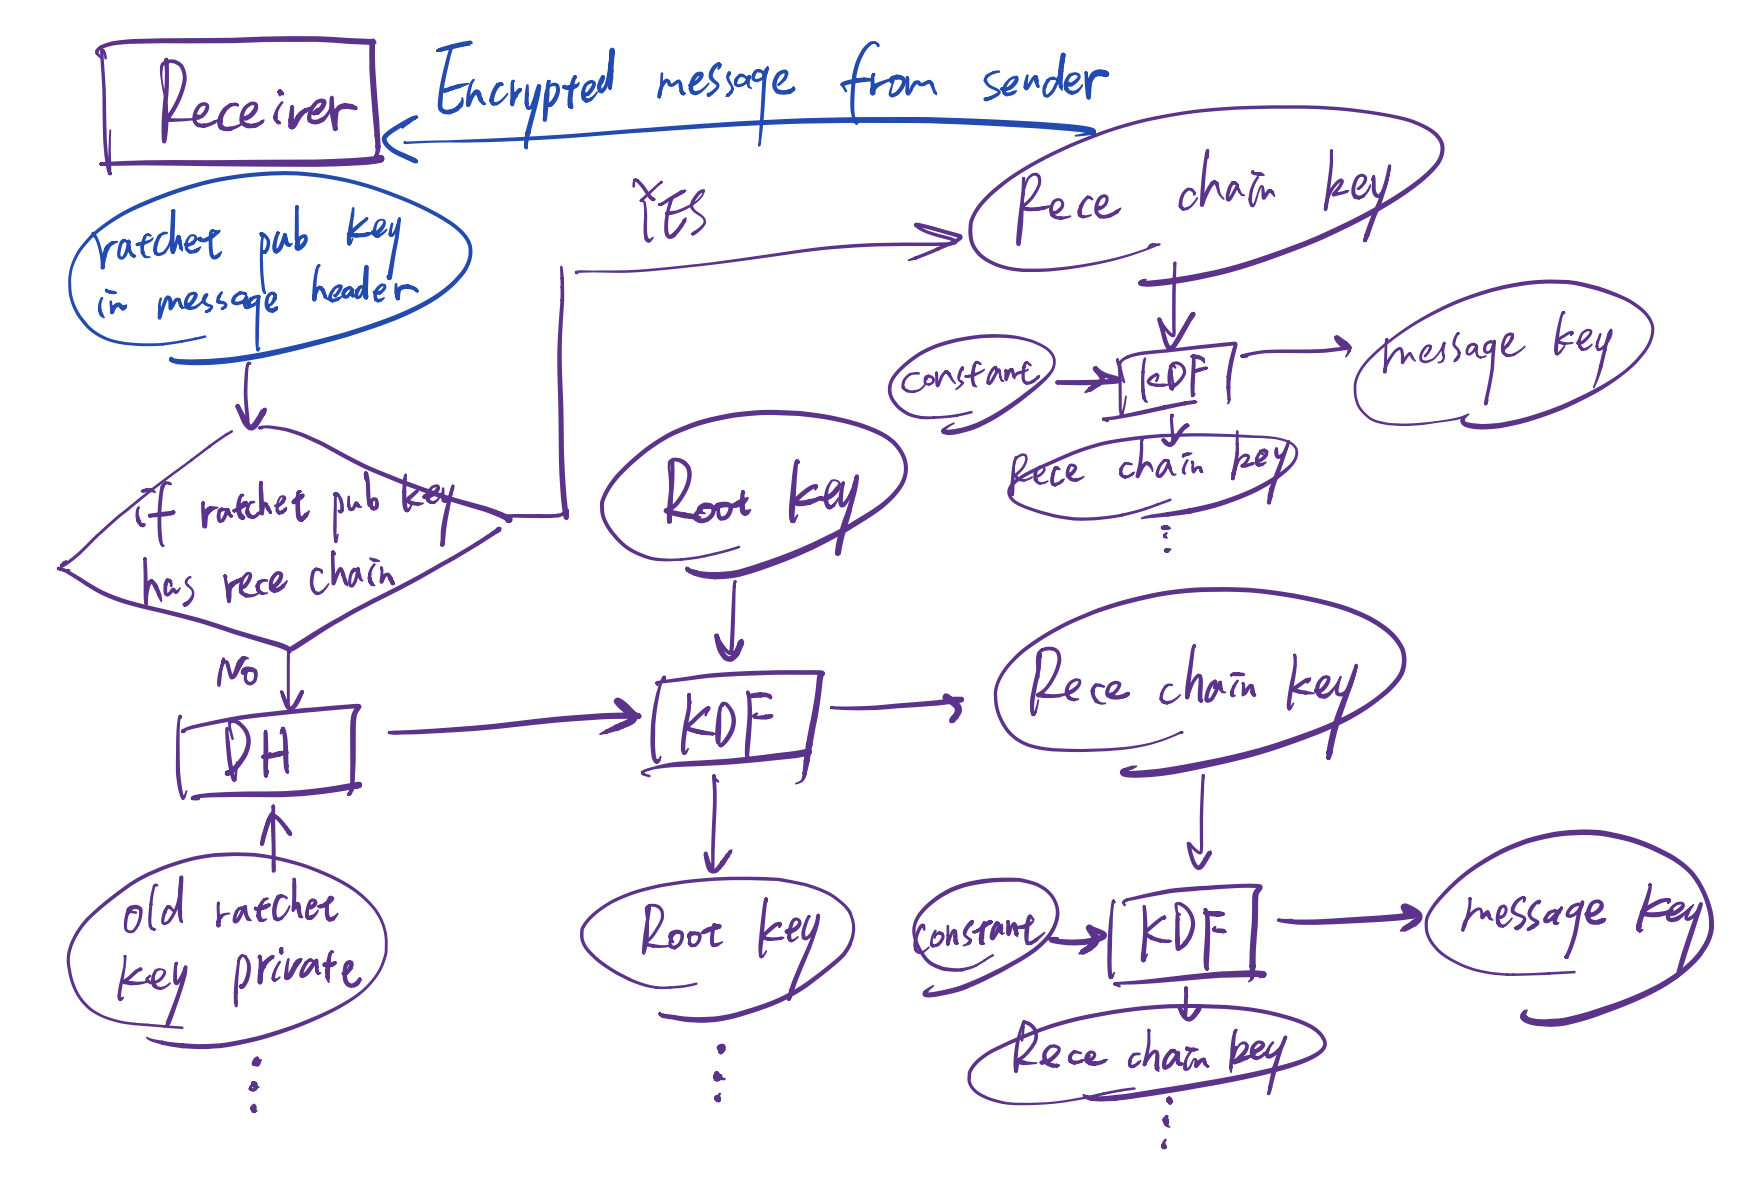
\includegraphics[scale=.5]{../3-Background/resources/DH-rece.png}\\
Figure 4.15: \textit{The fingerprint of pairwise chat on Alice side}
\end{center}

\begin{center}
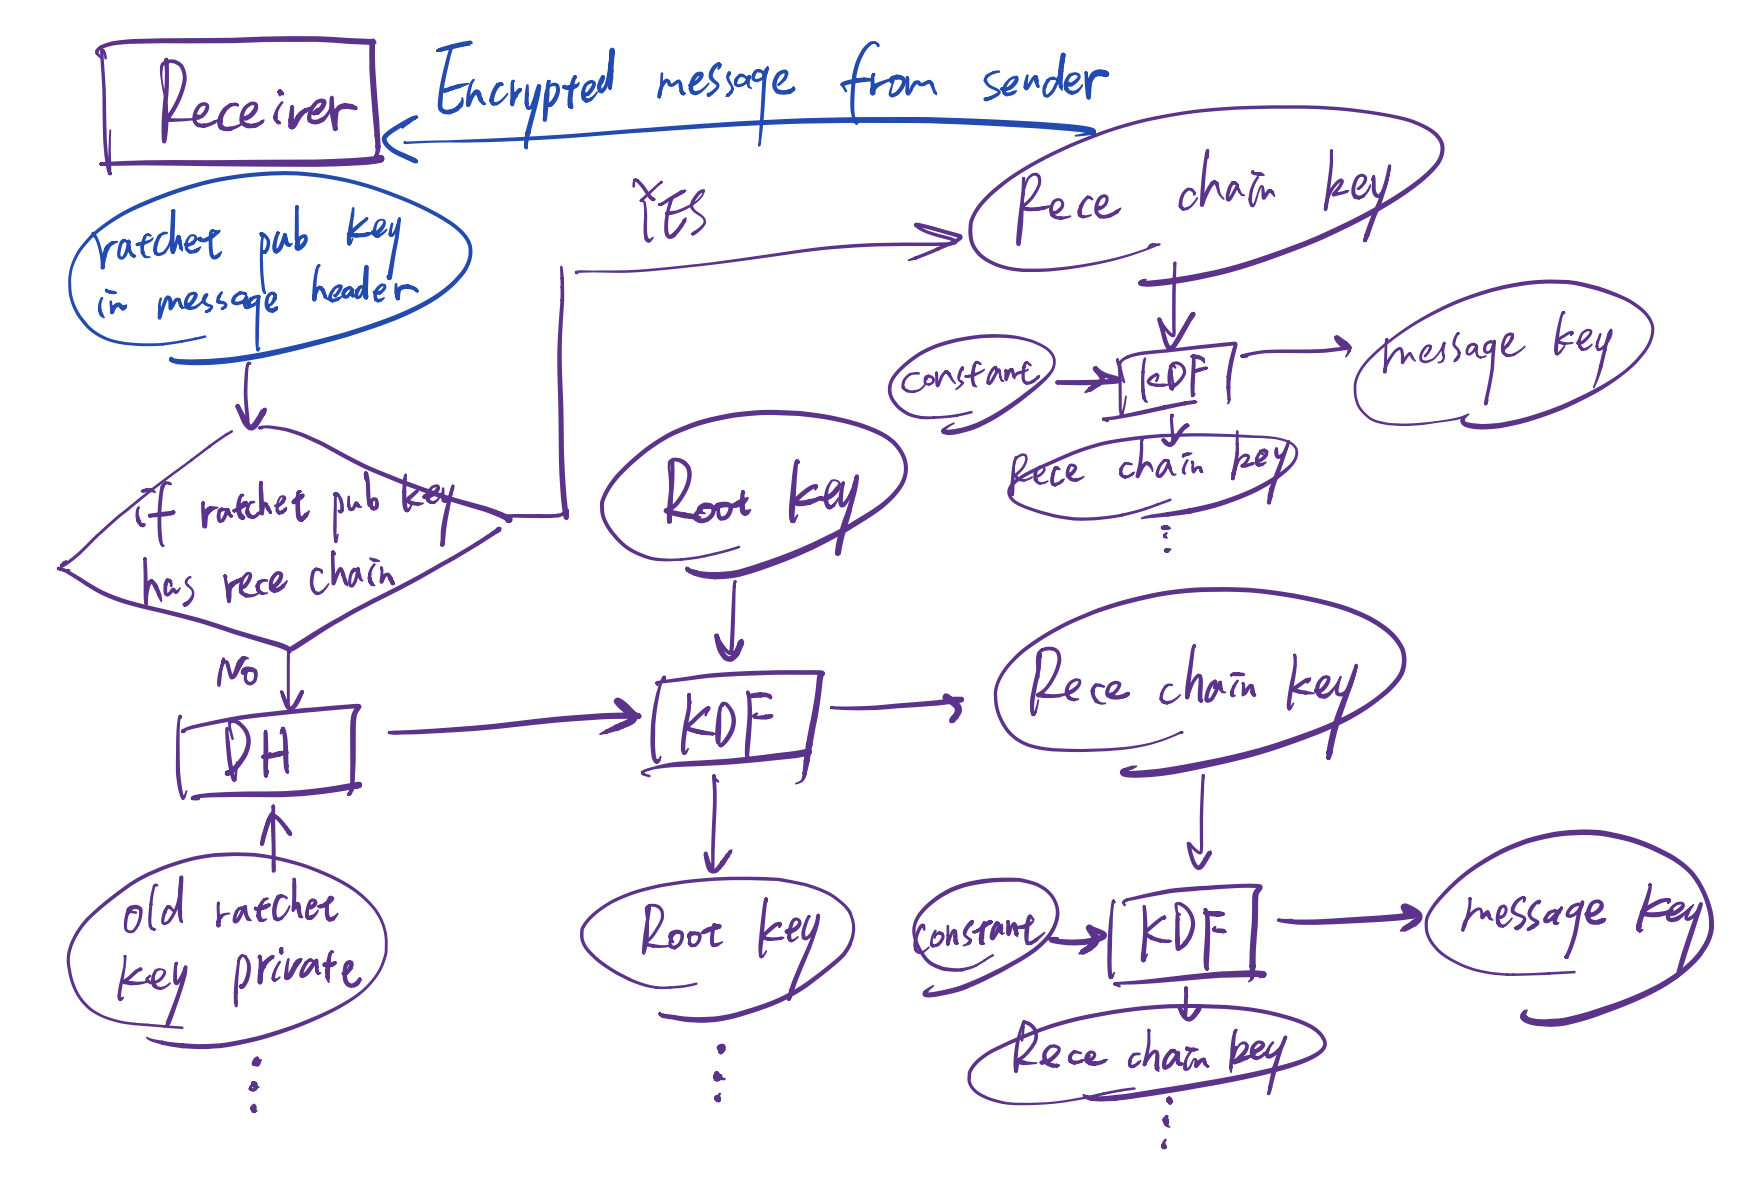
\includegraphics[scale=.5]{../3-Background/resources/DH-rece.png}\\
Figure 4.16: \textit{The fingerprint of pairwise chat on Bob side}
\end{center}

\end{enumerate}

\subsection{Project management}
The development of the project is completed within three months, so planning a proper schedule is necessary. In the first three weeks, reading lots of papers and website resources is essential to have a deep understanding about the Signal Protocol. Then determining the requirements of users and the application specification is the precondition of implementation. Once the prototype is determined, the implementation could start to develop.

During implementing, having a proper git branch structure does more with less. All the new functions are developed in branch ZiyanWang, after the implementation and testing, the code would be merged to the master branch. This process could make sure the new added functions would not break down the whole system while developing. Sometimes finding the unexpected bug is usual during development, the tests could not cover all the aspects. When fixing the issues, the developing code could be stashed for not confusing the thinking.

Commit records of git is also useful during developing. Make sure every steps is small. For example, every new added function and every fixing of issues could be committed as a new record. That would make the code version clearer, once the system breaks down the project could roll back to the latest version without too much loss.

\subsection{Results and evaluation}
After all the implementation of new functions in the whole system, the chat system is upgraded to a secure E2EE chat system. The features of it include the pairwise chat, group chat, switching device and messages backup etc. Users could communicate with each other in secure based on Signal Protocol. To verify the Signal Protocol works correctly in this system, the message key obtained from the symmetric ratchet is printed in client after each encryption and decryption. Comparing two message keys of two parties is a clear proof of the implementation of Signal Protocol. The figure 4.17 and figure 4.18 present the printed message keys of one pairwise chat's two parties respectively.

\begin{center}
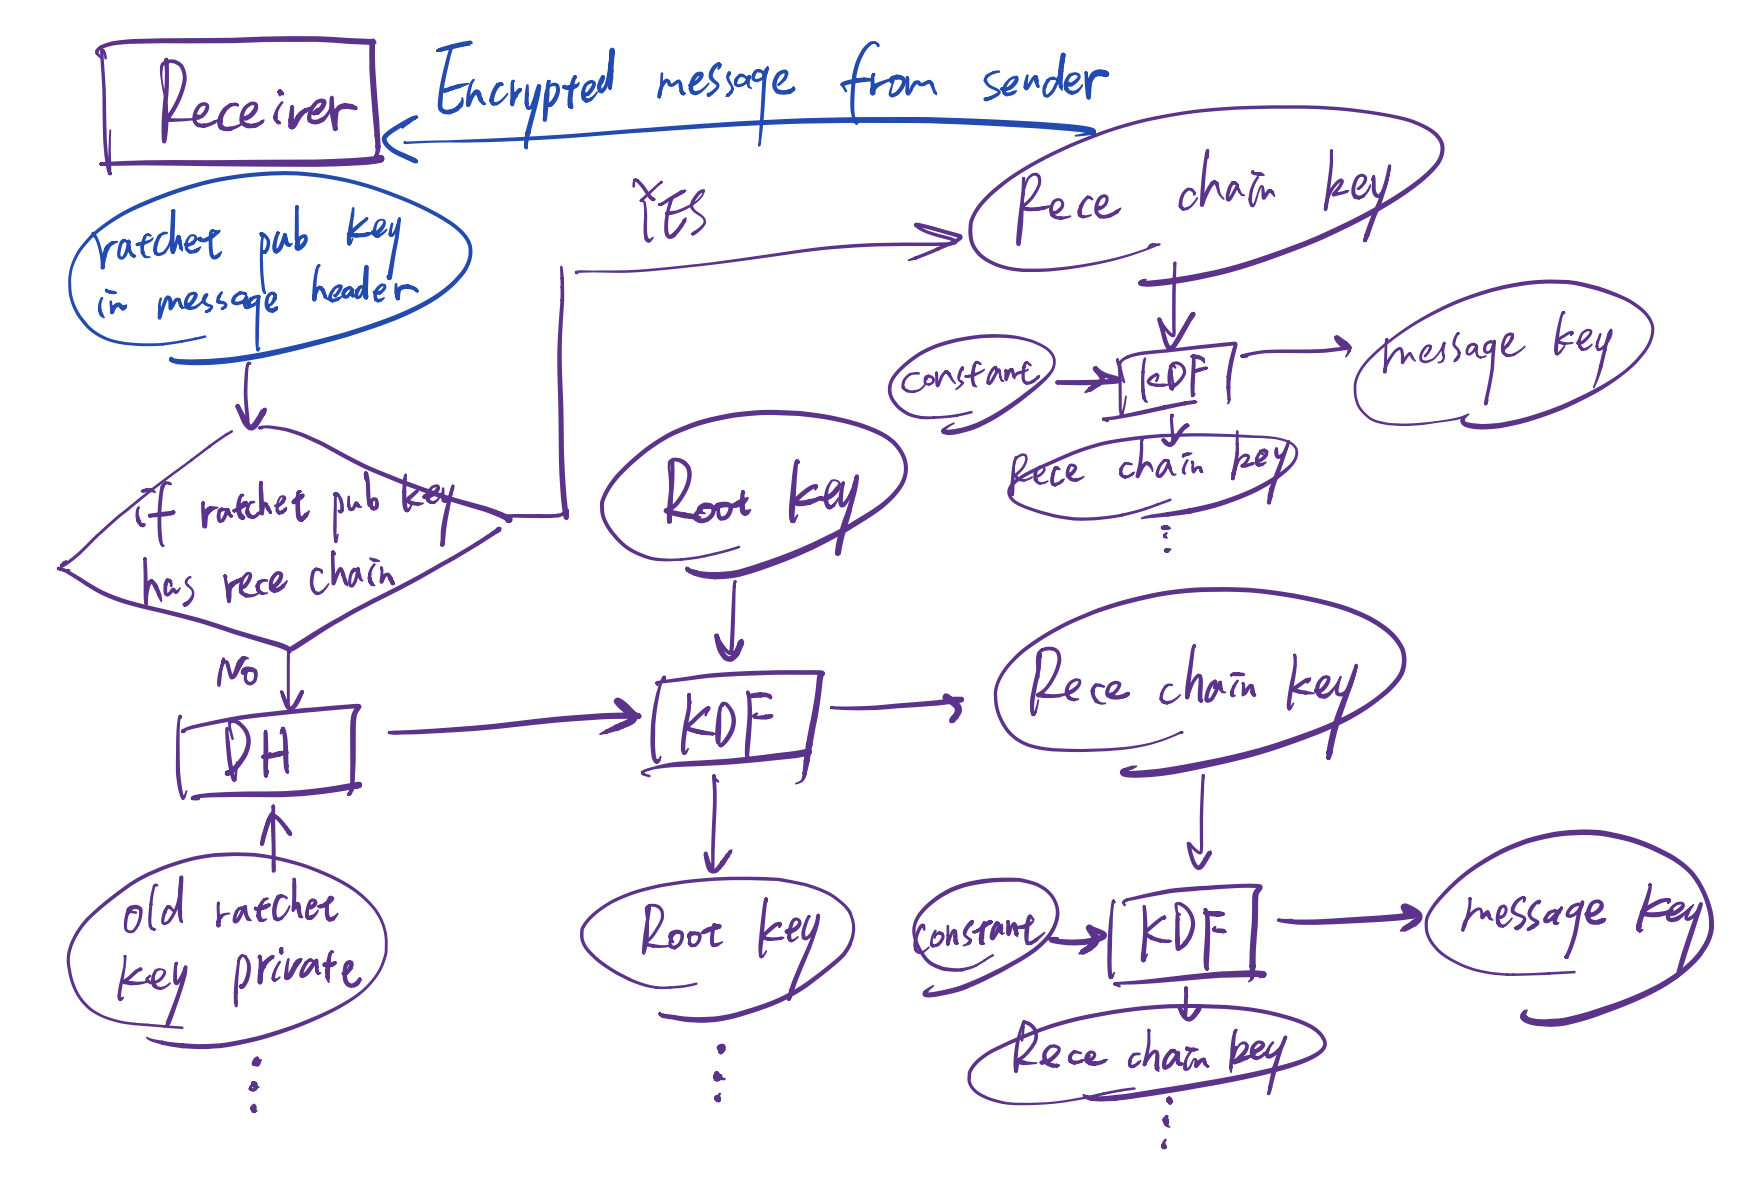
\includegraphics[scale=.5]{../3-Background/resources/DH-rece.png}\\
Figure 4.17: \textit{The message key after encryption on sender side}
\end{center}

\begin{center}
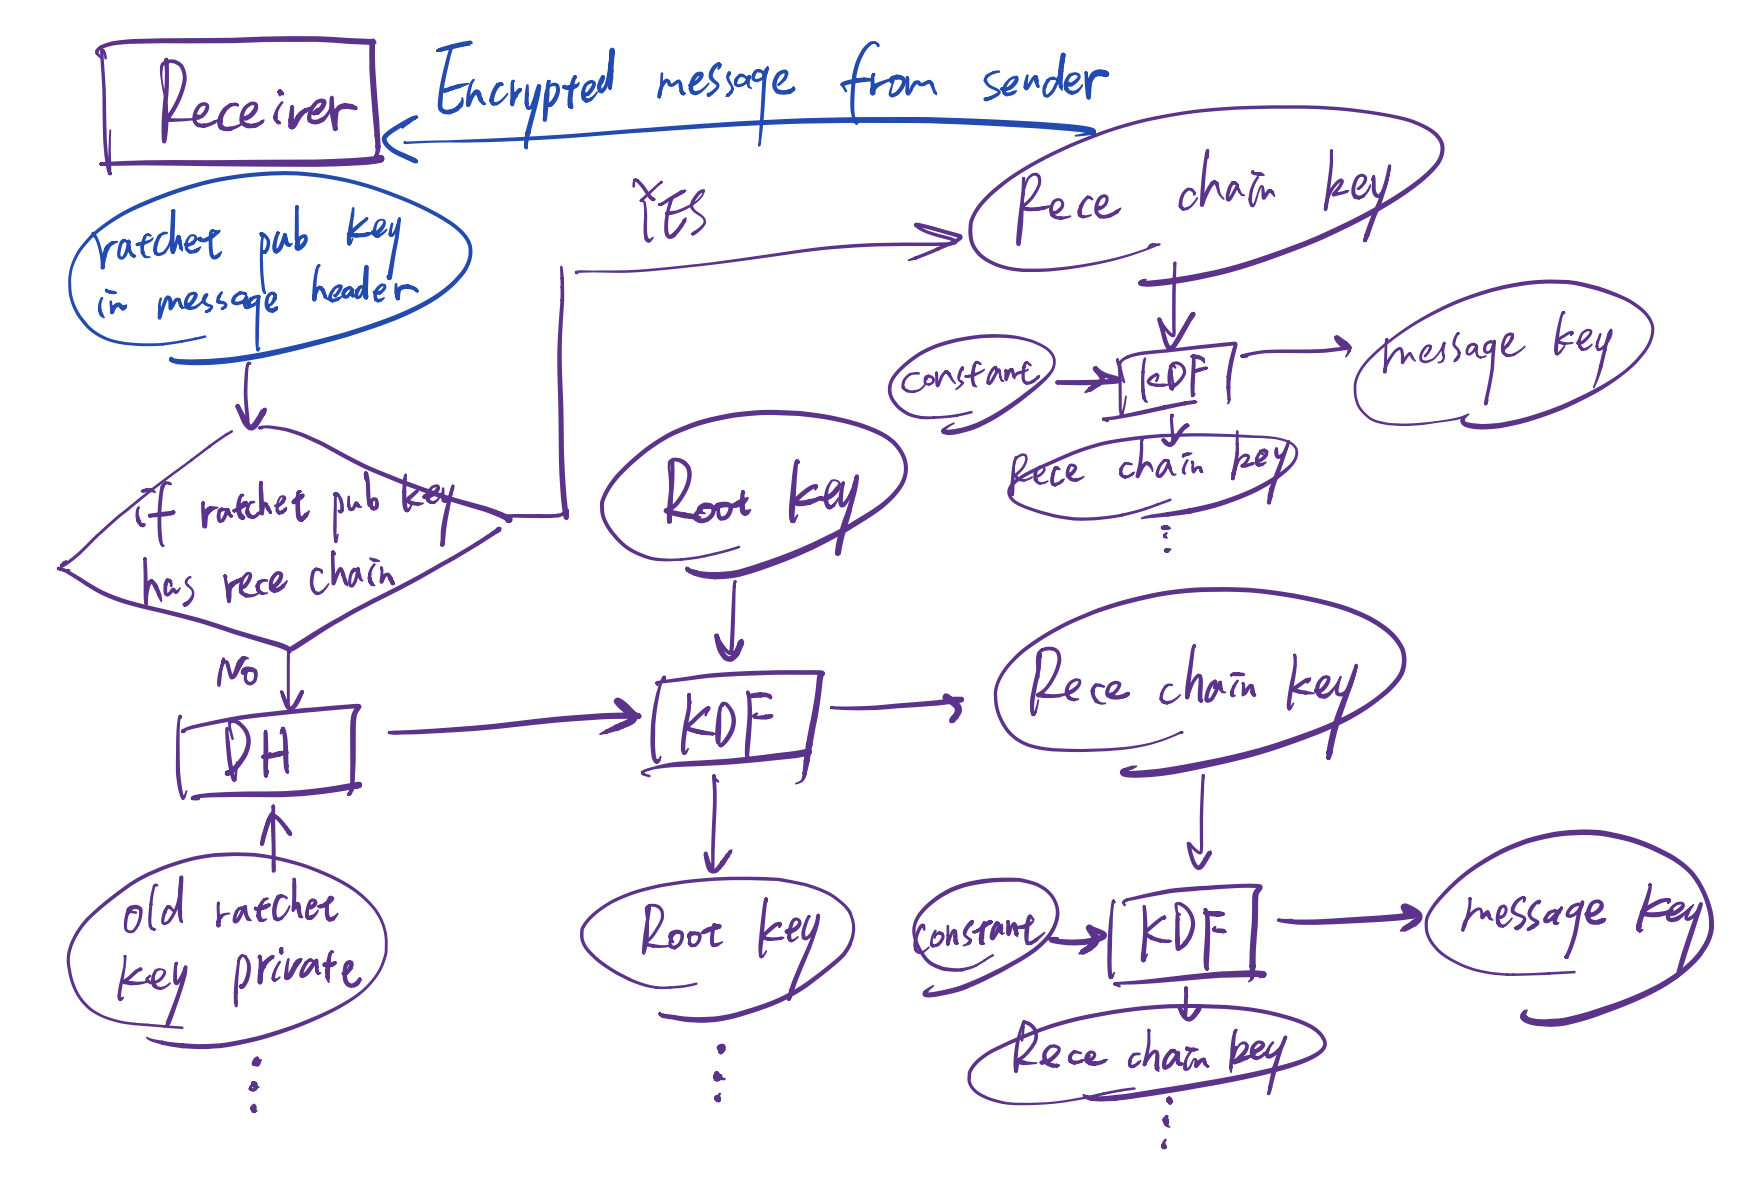
\includegraphics[scale=.5]{../3-Background/resources/DH-rece.png}\\
Figure 4.18: \textit{The message key after decryption on receiver side}
\end{center}

The final product basically accords with the initial design in terms of functions. After all implementation completed, the system could work correctly in pairwise chat, group chat and multi-device system etc.

There are still several defects that influence the robustness and performance of the system. For example, the system does not implement the SQL injection attack prevention system. The adversary could use the SQL inquiry flaw to get the user privacy. Also due to the IO structure of the previous system, the switching device function may not work as expected after a few times of continuous switches. As for the performance, the server verification user function inquires the data from database several times which causes the time performance issue. And since the thread pool is not used to handle the multi threads work allocation, the server may break down when the great amount of users login in together. Besides, because the server uses the SSH to connect to the database served by bham, the connection may be broken in a poor network environment which would cause the whole system down.

\clearpage